

\documentclass[english,11pt]{beamer}

\DeclareMathOperator{\Cov}{Cov}
\DeclareMathOperator{\Var}{Var}
\DeclareMathOperator{\E}{\mathbb{E}}
\DeclareMathOperator{\Proba}{\mathbb{P}}

\newcommand{\Covb}[2]{\ensuremath{\Cov\!\left[#1,#2\right]}}
\newcommand{\Eb}[1]{\ensuremath{\E\!\left[#1\right]}}
\newcommand{\Pb}[1]{\ensuremath{\Proba\!\left[#1\right]}}
\newcommand{\Varb}[1]{\ensuremath{\Var\!\left[#1\right]}}

% norm
\newcommand{\norm}[1]{\| #1 \|}

\newcommand{\indep}{\rotatebox[origin=c]{90}{$\models$}}





\usepackage{mathptmx,amsmath,amssymb,graphicx,bibentry,bbm,babel,ragged2e}

\makeatletter

\newcommand{\noun}[1]{\textsc{#1}}
\newcommand{\jitem}[1]{\item \begin{justify} #1 \end{justify} \vfill{}}
\newcommand{\sframe}[2]{\frame{\frametitle{#1} #2}}

\newenvironment{centercolumns}{\begin{columns}[c]}{\end{columns}}
%\newenvironment{jitem}{\begin{justify}\begin{itemize}}{\end{itemize}\end{justify}}

\usetheme{Warsaw}
\setbeamertemplate{footline}[text line]{}
\setbeamertemplate{headline}{}
\setbeamercolor{structure}{fg=purple!50!blue, bg=purple!50!blue}

\setbeamersize{text margin left=15pt,text margin right=15pt}

\setbeamercovered{transparent}


\@ifundefined{showcaptionsetup}{}{%
 \PassOptionsToPackage{caption=false}{subfig}}
\usepackage{subfig}

\usepackage[utf8]{inputenc}
\usepackage[T1]{fontenc}

\usepackage{multirow}

\usepackage{mdframed}


%\AtBeginSection[]
%{
%  \begin{frame}
%  \frametitle{Integrating urban models and theories}
%  \tableofcontents[currentsection]
%  \end{frame}
%}

\makeatother

\begin{document}



% title FRCCS
%\title{Multi-modeling urban systems dynamics to explore sustainability trade-offs}
% title UGI-Urban
\title{Trade-offs between sustainable development goals in systems of cities}
% same title ERSA (TRSA-ABC)

\author{J.~Raimbault$^{1,2,3,4}$ and D.~Pumain$^4$\\
\texttt{juste.raimbault@ign.fr}
}


\institute{$^{1}$LASTIG, Univ Gustave Eiffel, IGN-ENSG\\
$^{2}$CASA, UCL\\
$^{3}$UPS CNRS 3611 ISC-PIF\\
$^{4}$UMR CNRS 8504 G{\'e}ographie-cit{\'e}s
}


%\date{French Regional Conference on Complex Systems 2022\\
%June 22th 2022\\\bigskip
%
\includegraphics[width=0.1\textwidth]{figures/logoFRCCS}
%}

%\date{2022 IGU Urban Commission Annual Meeting\\
%July 25th 2022
%}

\date{ERSA 2022 - TRSA ABC\\
August 23rd 2022
}


%Cities and urban systems appear as key elements to tackle the challenges of sustainability, as they combine negative and positive externalities on multiple dimensions, including the envi- ronmental and the socio-economic aspects. Besides, empirical, modeling and theoretical evidence suggest the existence of trade-offs between different Sustainable Development Goals (SDGs) in urban systems. We propose in this contribution to investigate such trade-offs from a modeling perspective. Building on previous work benchmarking macroscopic models of urban systems dy- namics (Raimbault, Denis & Pumain, 2020) based on the evolutionary urban theory (Pumain, 2018), we introduce in a multi-modeling approach the coupling of several layers for complemen- tary dimensions of urban systems. More precisely, we combine an innovation diffusion model, an economic exchange model, and a transportation network model, with a common core of population dynamics. The resulting macroscopic model is parametrised on population data for large urban systems worldwide (Pumain et al., 2015), and integrated into the OpenMOLE platform for model exploration and validation (Reuillon et al., 2013). This allows running a multi-objective optimi- sation algorithm on proxy indicators for multiple goals: innovation (goal 8 “Economic Growth”), transportation network (goal 9 “Infrastructure”), economic inequalities between cities (goal 10 “Inequalities”), and greenhouse gases emissions (goal 13 “Climate”). We therein confirm the ex- istence of trade-offs in macroscopic urban dynamics by obtaining Pareto front between these four dimensions. Future perspectives include the extension to multi-scale models to include intra-urban dimensions (and some aspects of goal 11 “Sustainable cities and societies”) and further model in- tegration to account for other dimensions and goals. Altogether, this horizontal and vertical model integration approach builds the foundations towards multi-scale policies for sustainable territories (Raimbault, 2021).



\frame{\maketitle}


\section{Introduction}


% striking image - intro?
% Mike: cities as transitionnal state?

\sframe{Cities and SDGs}{

%\justify

\textbf{SDG 11}: ``Make cities and human settlements inclusive, safe, resilient, and sustainable'' \cite{nations2015sustainable}

\bigskip

$\rightarrow$ Cities as a transition state? \cite{batty2018inventing} Incubators of social change and innovation, both the source and solution to sustainability issues? \cite{pumain2010theorie}

\bigskip

$\rightarrow$ Environmental Kuznet Curve hypothesis \cite{dinda2004environmental, stern2004rise}: inverted U-shaped relationship between environmental impact and income per-capita; not validated empirically \cite{harbaugh2002reexamining}

\bigskip

$\rightarrow$ Trade-offs between SDGs in urban systems \cite{viguie2012trade}


}

\sframe{Bi-objective trade-offs}{

\centering

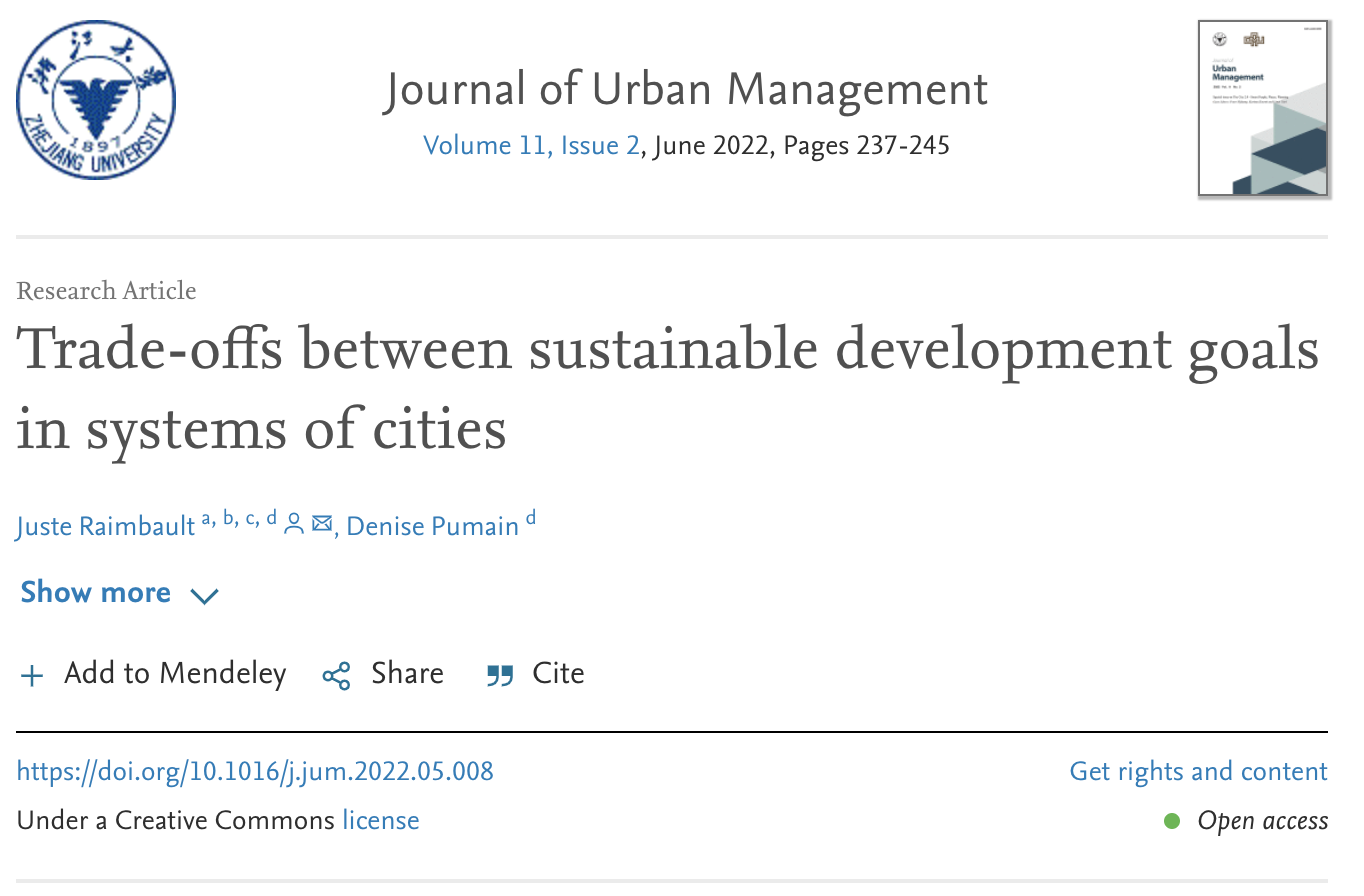
\includegraphics[height=0.8\textheight]{figures/jum_paper.png}

}

\sframe{Research objective}{

$\rightarrow$ More dimensions and SDGs with trade-offs?

\medskip

$\rightarrow$ Several models introduced with the evolutionary urban theory \cite{pumain2018evolutionary} tackle complementary dimensions (see \cite{raimbault2020empowering} for a benchmark)


\bigskip
\bigskip

\textbf{Research objective: }

\smallskip

\textit{Couple several models for complementary dimensions of urban dynamics (innovation, economic exchanges, infrastructure) into a multi-model for the dynamics of urban systems at the macroscopic scale, to explore trade-offs between SDGs in synthetic systems of cities.}


}







\section{Innovation diffusion model}



\sframe{Innovation diffusion and urban dynamics}{

\textbf{Exploration of trade-offs with two dimensions: urban evolution model} \cite{raimbault2022trade}

\bigskip
\bigskip

$\rightarrow$ \textbf{Innovation diffusion} is a crucial process in artificial life evolutionary systems and open-ended evolution \cite{bedau2000open}

\medskip

$\rightarrow$ Artificial societies used to study the dynamics of innovation \cite{zenobia2009artificial}

\medskip

$\rightarrow$ Innovations diffuse hierarchically in systems of cities \cite{hagerstrand1968innovation}, potential explanation of urban scaling laws \cite{pumain2006evolutionary}

\bigskip

\textit{Innovation diffusion as a privileged entry to understand urban evolution}


}



\sframe{Model rationale}{


\begin{itemize}
	\item Agents are cities, macroscopic scale (regional, country, continental) and long time scales (century)
	\item Cities characterised by their size in terms of population; genome as adoption proportions of innovations (social or technological) for each city (one single dimension to simplify)
	\item Following \cite{favaro2011gibrat}, attractivity of cities due to level of innovation drive their population growth through spatial interactions; innovation diffuse through an other spatial interaction model \cite{fotheringham1989spatial}
	\item Mutations occur in cities as new innovations appear
\end{itemize}

}




\sframe{Model description}{
\centering
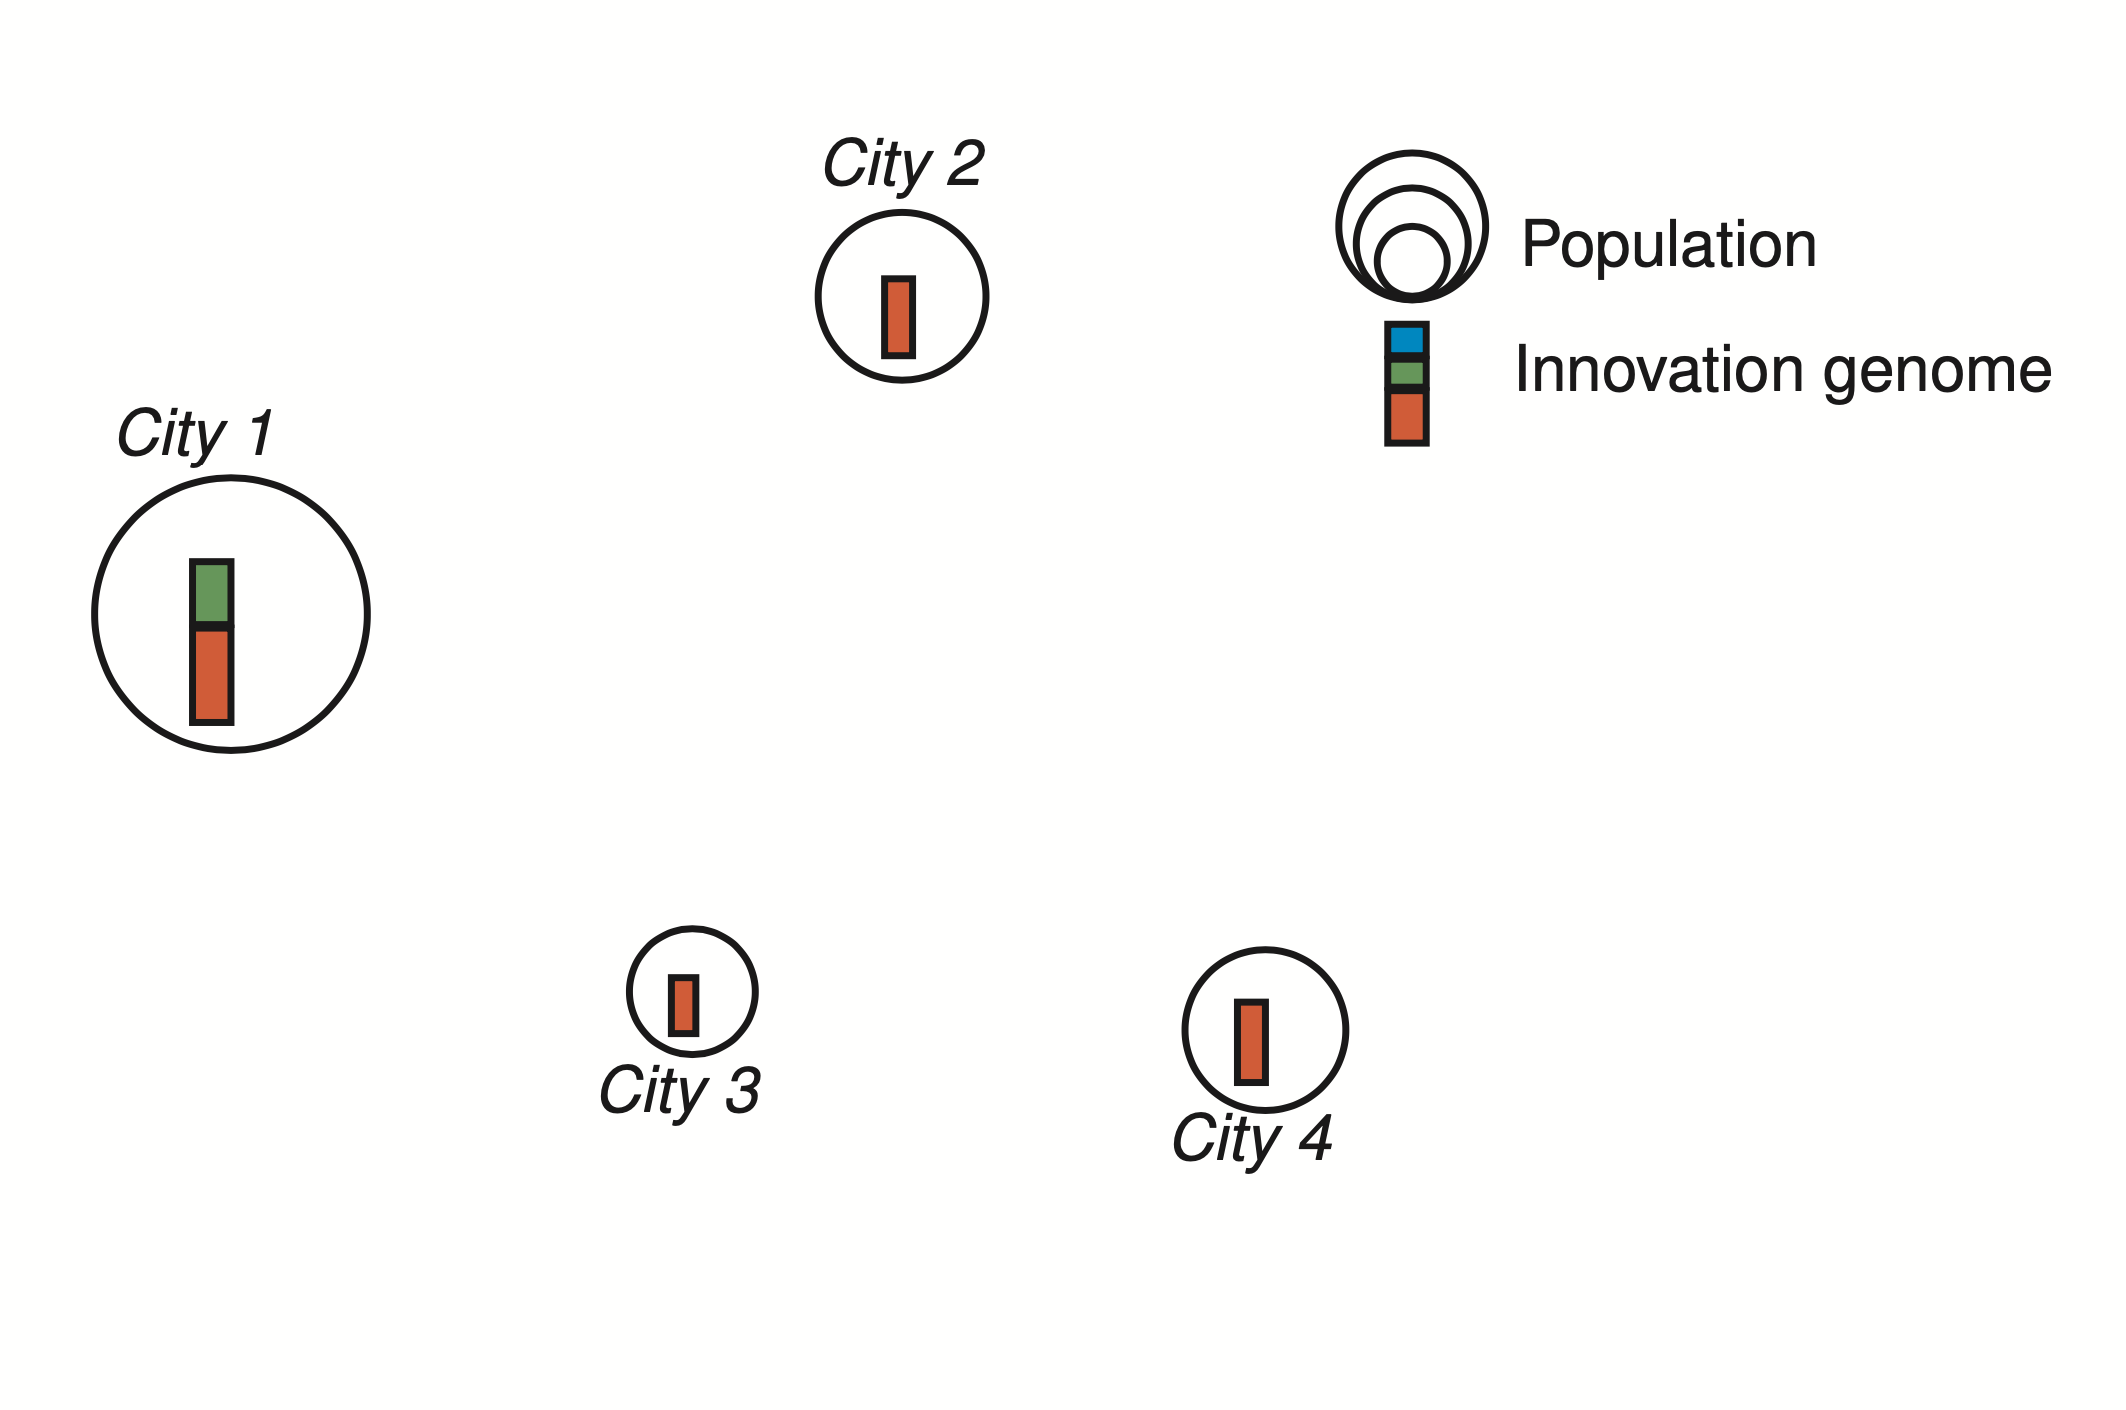
\includegraphics[width=\linewidth]{figures/model_1.png}
}

\sframe{Model description}{
\centering
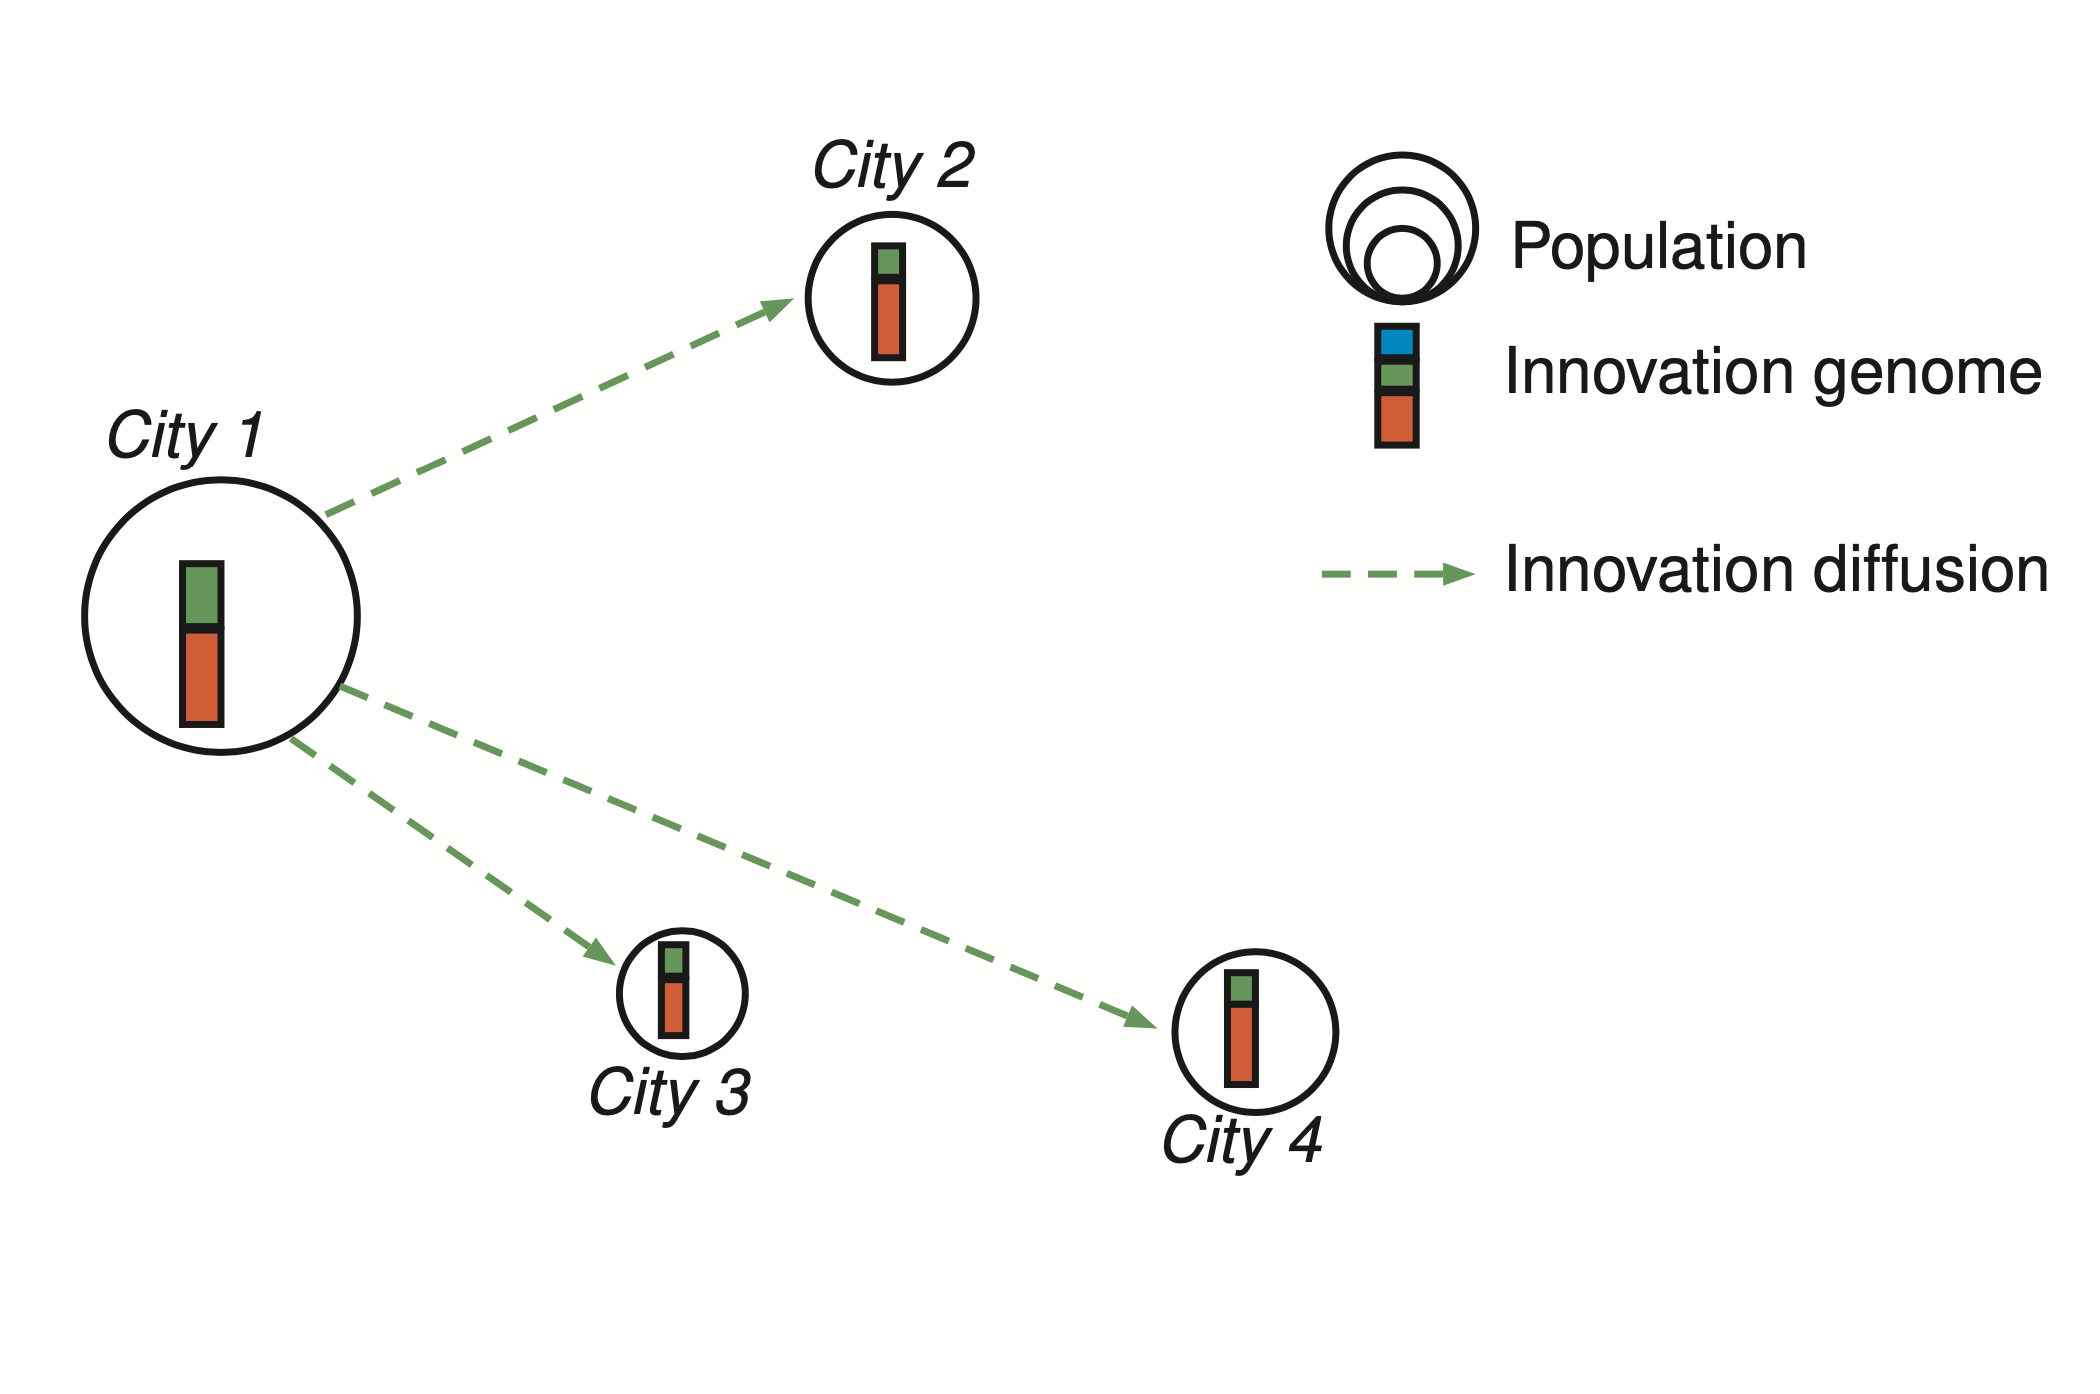
\includegraphics[width=\linewidth]{figures/model_2.png}
}

\sframe{Model description}{
\centering
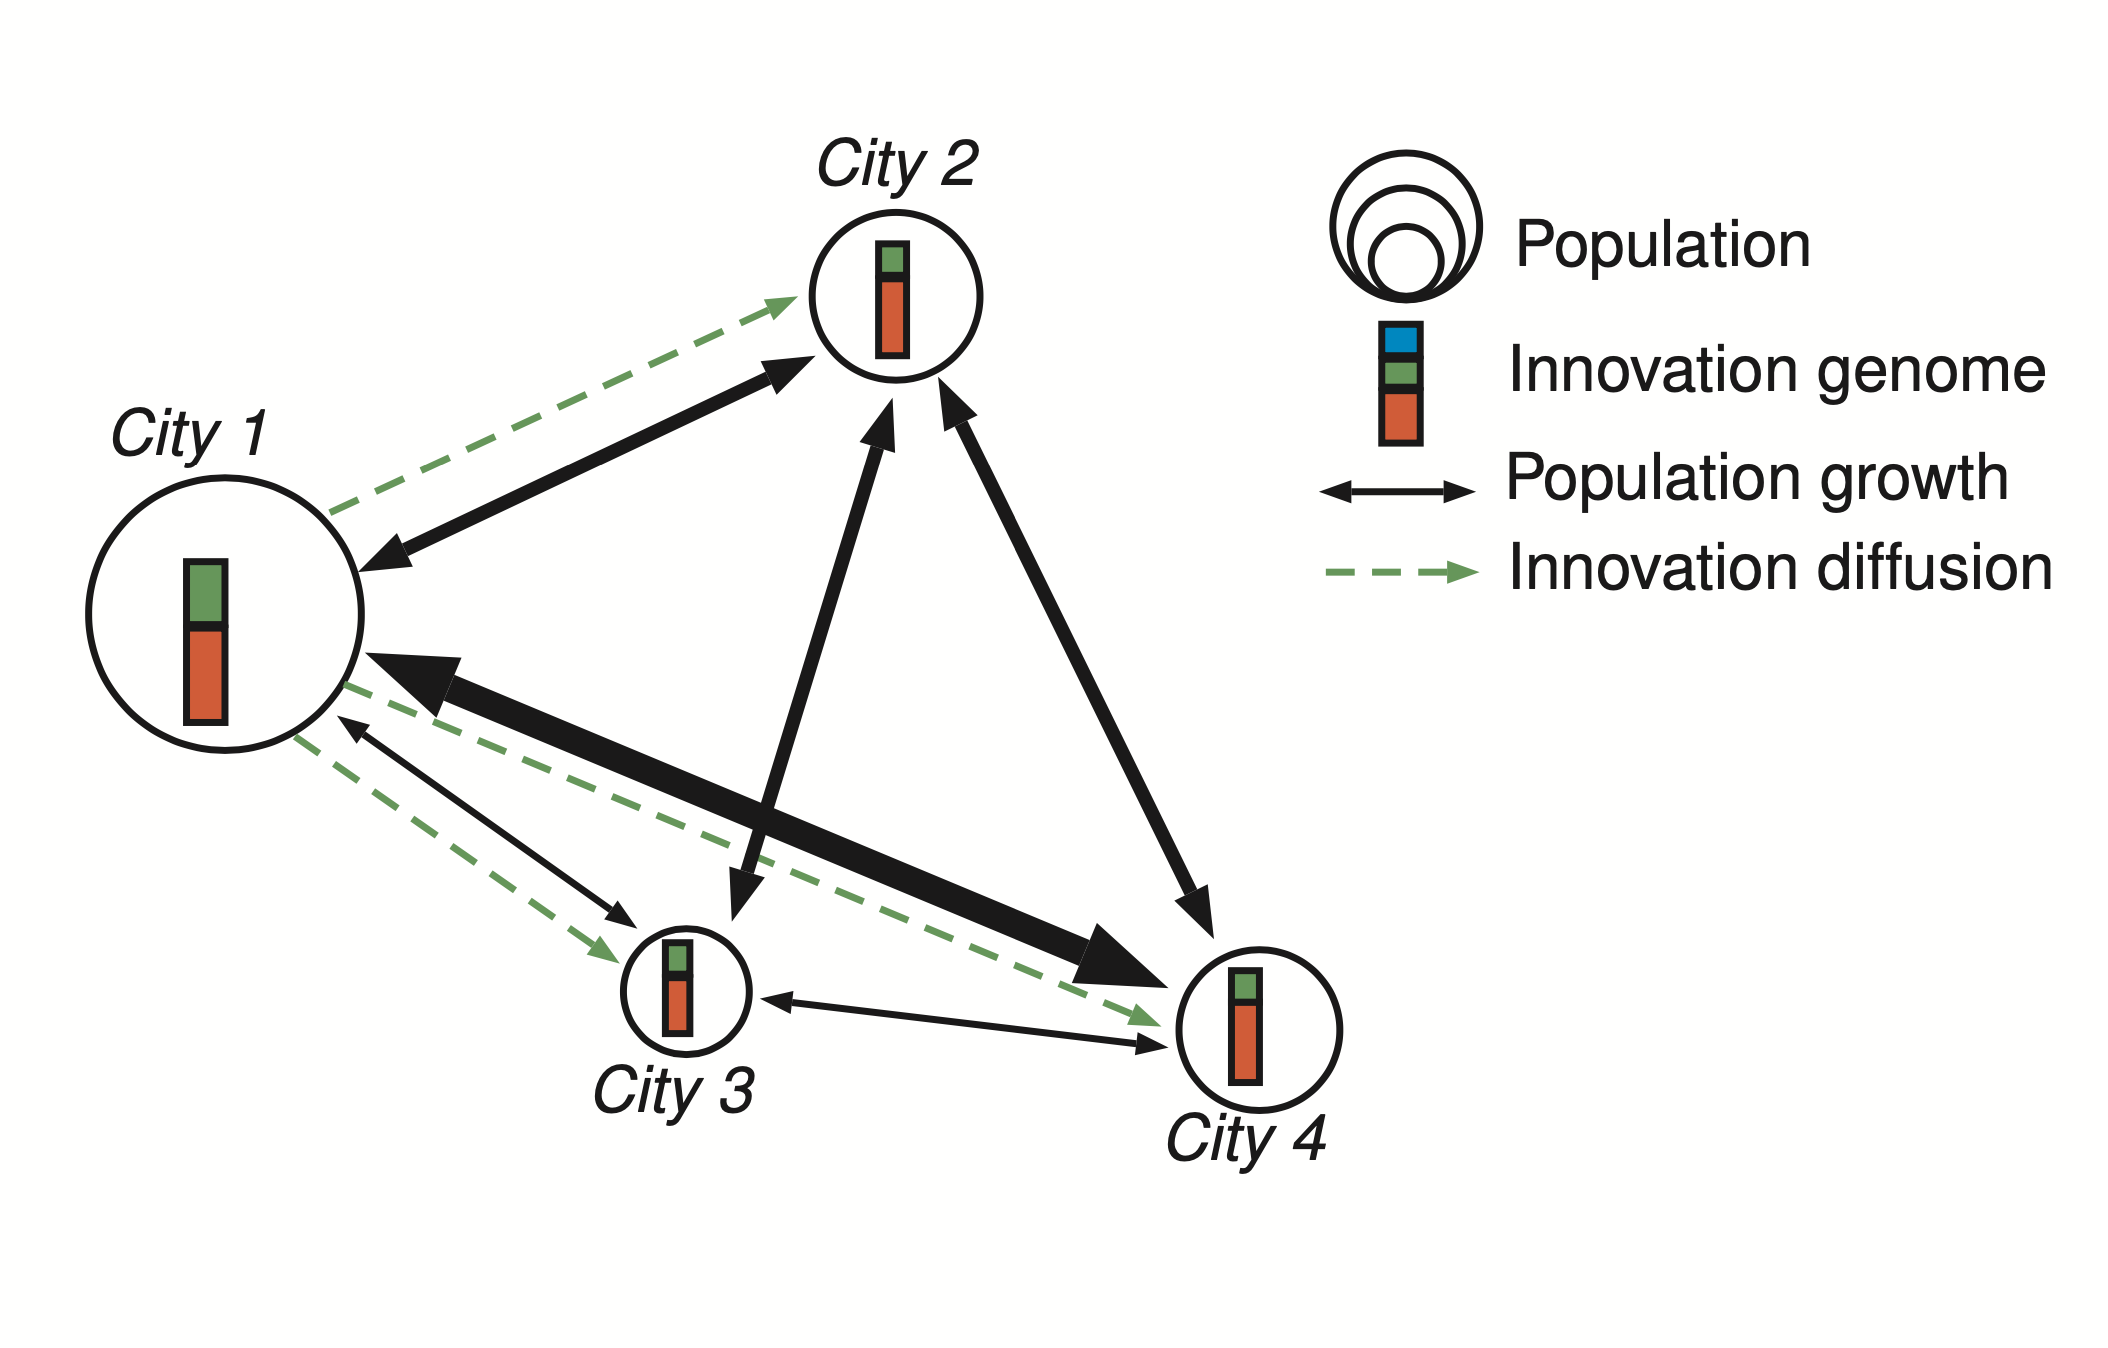
\includegraphics[width=\linewidth]{figures/model_3.png}
}

\sframe{Model description}{
\centering
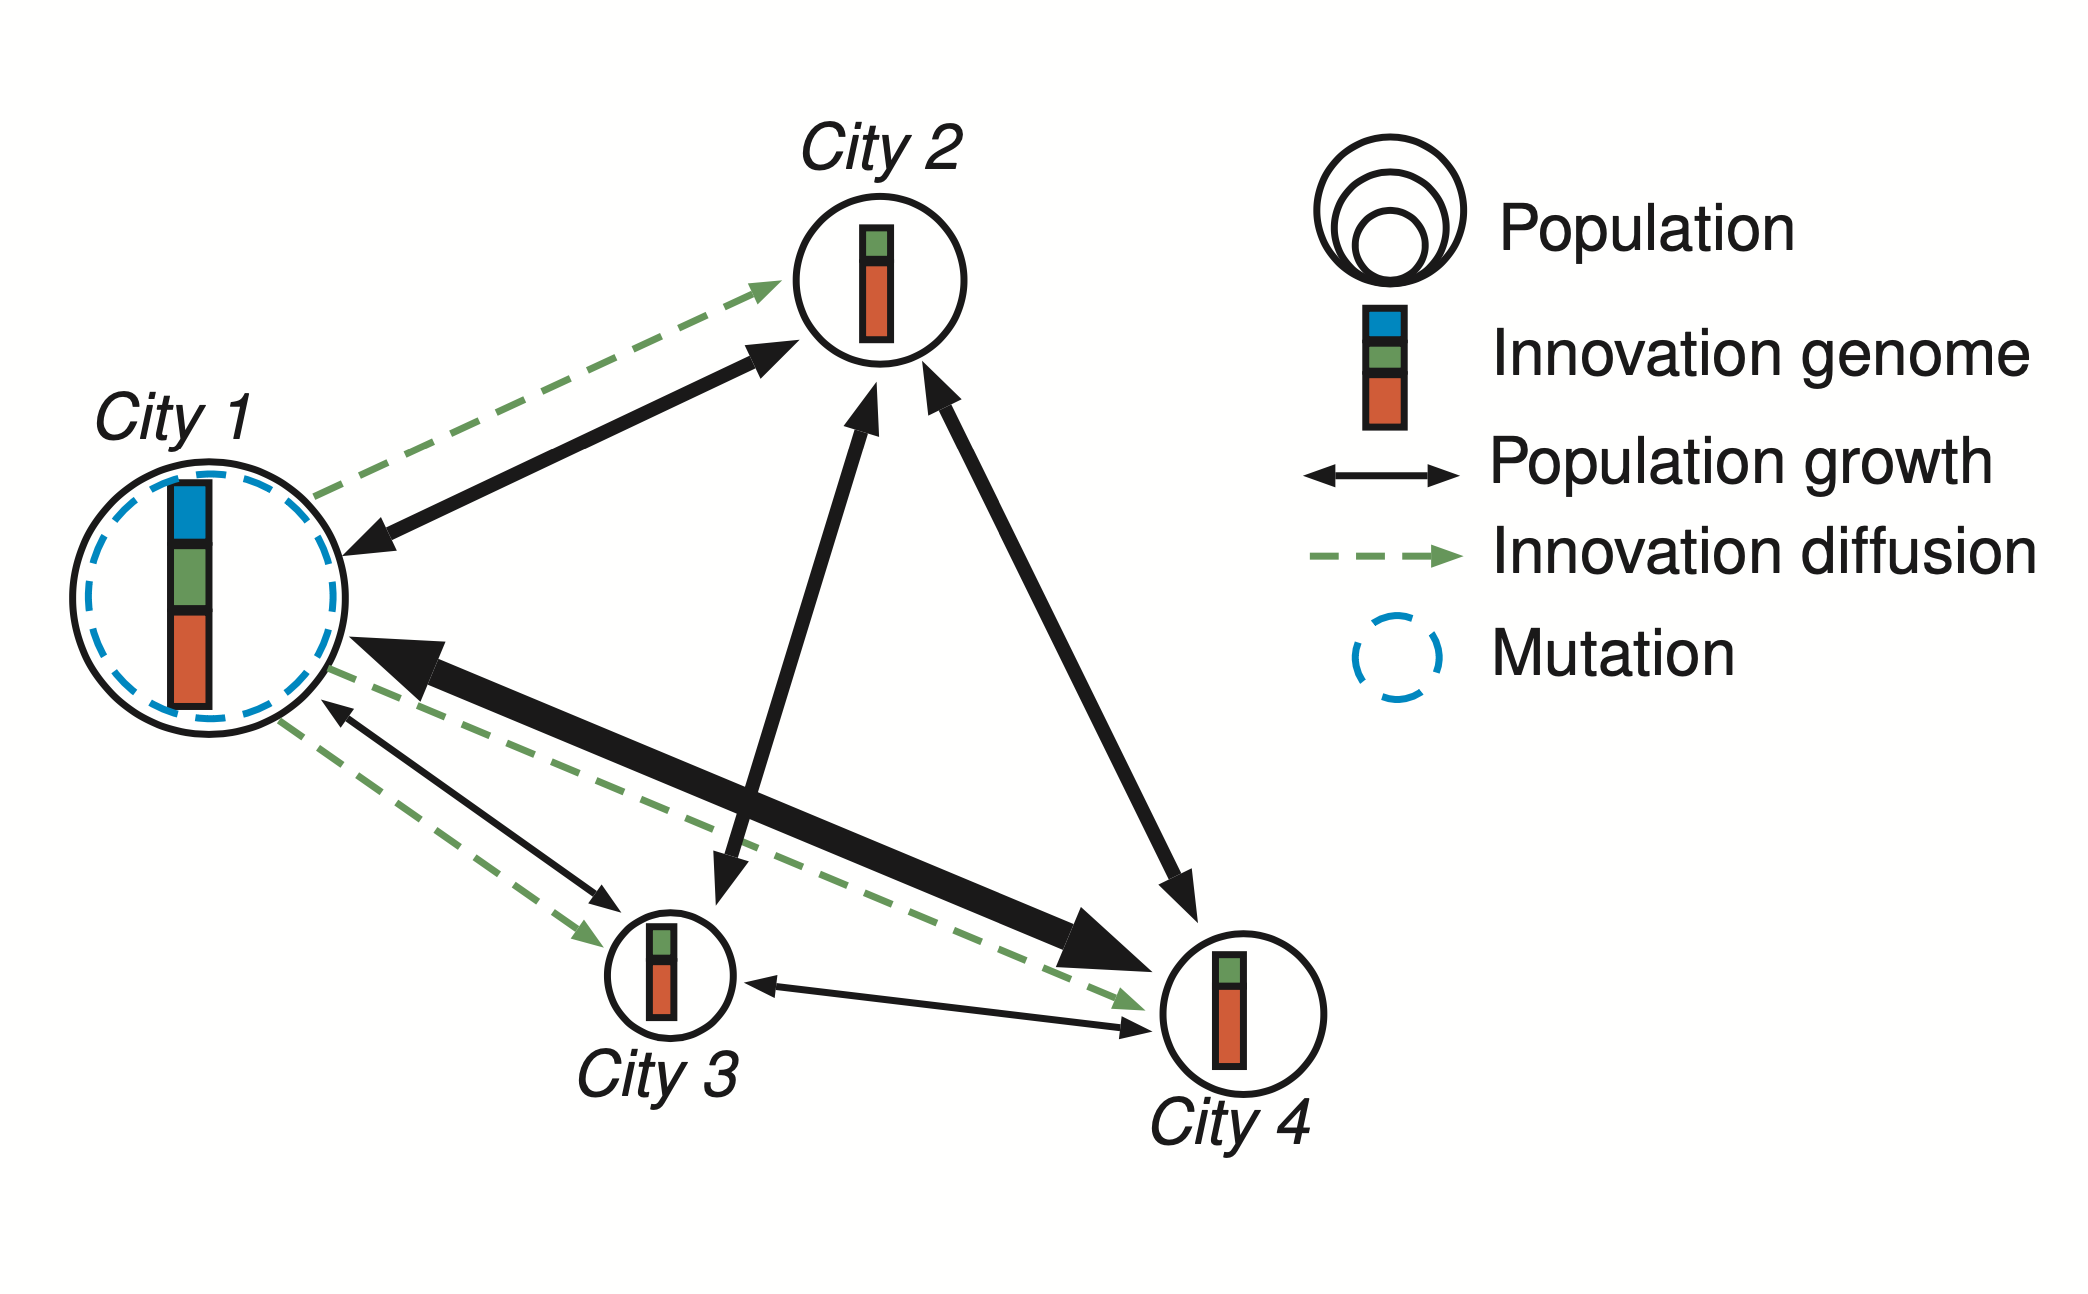
\includegraphics[width=\linewidth]{figures/model_4.png}
}



\sframe{Model formalisation}{


At each time step, with $P_i \left(t\right)$ population, $\delta_{c,i}\left(t\right)$ genome, $u_c$ utility of innovation, $p_{c,i,t}$ share of total population adopting innovation $c$ in city $i$
\begin{enumerate}
	\item Crossover through the diffusion of innovations
	\[
	\delta_{c,i,t} \textrm{ = } \frac{\sum_j p_{c,j,t-1}^{\frac{1}{u_c}} \cdot \exp{\left(-\frac{d_{ij}}{d_I}\right)}}{\sum_c \sum_j p_{c,j,t-1}^{\frac{1}{u_c}} \cdot \exp{\left(-\frac{d_{ij}}{d_I}\right)}}	
	\]
	\item Population growth through spatial interactions $P_i\left(t\right) - P_i\left(t-1\right) \textrm{ = } w_I\cdot \sum_j \frac{V_{ij}}{<V_{ij}>}$ with
	\[ 
	V_{ij} \textrm{ = } \frac{P_{i}\left(t-1\right) \cdot P_{j}\left(t-1\right)}{\left(\sum_k P_k\left(t-1\right)\right)^2} \cdot \exp{\left(-\frac{d_{ij}}{d_G} \cdot \prod_c \delta_{c,i,t}^{\phi_{c,t}}\right)}
	\]
	and $\phi_{c,t} \textrm{ = } \sum_i \delta_{i,c,t}\cdot P_i\left(t-1\right) /\sum_{i,c} \delta_{i,c,t}\cdot P_{i}\left(t-1\right)$
	\item Mutations with innovations introduced with probability $\beta \cdot \left(P_i \left(t\right) / \max_k P_k \left(t\right)\right)^{\alpha_I}$ and an initial penetration rate $r_0$; new utility $u_c$ randomly distributed (normal or log-normal) with average current average utility and standard deviation a given parameter $\sigma_U$
\end{enumerate}



}


%\sframe{Model indicators}{

%\begin{itemize}
%	\item Average diversity
%	\[
%	D \textrm{ = } \frac{1}{t_f \textrm{+} 1} \sum_{t\textrm{=}0}^{t_f} \left(1 - \sum_{i,c} \left(p_{c,i,t}\right)^2 \right)	
%	\]
%	\item Average utility
%	\[
%	U \textrm{ = } \frac{1}{t_f \textrm{ + } 1} \sum_{t \textrm{=}0}^{t_f} \sum_{i,c} \delta_{c,i,t} u_c 
%	\]
%	\item Innovatitivity 
%	\[
%	I \textrm{ = } \frac{\max c}{N\cdot \left(t_f \textrm{ + } 1\right)}
%	\]
%	\item Population trajectories, summarized by final hierarchy \cite{raimbault2020unveiling}
%\end{itemize}
%}



\sframe{Synthetic configurations}{

Model applied on synthetic systems of cities (so that conclusions are independent of geographical contingencies \cite{raimbault2019space}):

\medskip

\begin{itemize}
	\item random positions and rank-size hierarchy $P_i \left(0\right) = \frac{P_{max}}{i^{\alpha_0}}$ with $\alpha_0 = 1.0$ and $P_{max} = 100,000$
	\item regional urban system scale: $N = 30$ cities
	\item simulated for $t_f = 50$ macroscopic time steps (order of magnitude of a century)
\end{itemize}



}



\sframe{Model parameters for the innovation model}{

\centering

	\begin{tabular}{|l|l|l|l|l|l|}
	\hline
	Parameter & Not. & Process & Range & Def. \\ \hline
	Number of cities & $N$ & Spatial scale & $[10 ; 100]$ & $30$\\
	Initial hierarchy & $\alpha_0$ & System of cities & $[0.5 ; 2.0]$ & $1$\\
	Initial population & $P_{max}$ & System of cities & $[10^4 ; 10^7]$ & $10^5$\\
	Simulation steps & $t_f$ & Temporal scale & $[10 ; 100]$ & $50$\\
	Growth rate & $w_I$ & Pop. growth & $[0.001 ; 0.01]$ & $0.005$\\\hline
	Gravity range & $d_G$ & Crossover & $[0 ; 2]$ & $1$\\
	Innovation range & $d_I$ & Crossover & $[0 ; 2]$ & $1$\\
	Innovation rate & $\beta$ & Mutation & $[0 ; 1]$ & $0.5$\\
	Innovation hierarchy & $\alpha_I$ & Mutation & $[0 ; 2]$ & $1$\\
	Innov. utility std. & $\sigma_U$ & Mutation & $\left[ 0.7;2\right]$ & $1$\\
 	Penetration rate & $r_0$ & Mutation & $\left[0.1;0.9\right]$ & $0.5$\\
	Utility type & - & Mutation & \{n;ln\}& ln \\
	\hline
	\end{tabular}


}



\sframe{Implementation}{

\justify

Model implemented in \texttt{scala}; relatively large parameter space; integration into the \texttt{spatialdata} scala library for spatial sensitivity analysis \cite{raimbault2020scala}

\medskip

$\rightarrow$ integration into the OpenMOLE model exploration open source software \cite{reuillon2013openmole}

\begin{center}

\includegraphics[height=0.13\textheight]{figures/iconOM.png}

\includegraphics[height=0.13\textheight]{figures/openmole.png}
\end{center}


\textit{Enables seamlessly (i) model embedding; (ii) access to HPC resources; (iii) exploration and optimization algorithms}

\medskip

\url{https://openmole.org/}


}




\sframe{Trade-offs between SDGs}{

\justify

$\rightarrow$ \textit{Which trade-offs between innovation (SDG 9: innovation) and emissions (SDG 14: climate) in systems of cities?}

\bigskip

Application of the urban evolution model, optimising with NSGA2 for conflicting objectives in synthetic systems of cities:

\medskip

\begin{enumerate}
   \item total utility of innovations 
 \[
 U = \sum_{t,i,c} \delta_{t,i,c} \cdot u_c
 \]
   \item gravity mobility flows as proxy for emissions
 \[
 E = \sum_{t,i,j} \frac{P_{t,i}P_{t,j}}{P_t^2} \cdot \exp\left(- d_{ij} / d_G\right)
 \]
 \end{enumerate}


}

\sframe{Trade-offs between SDG9 and SDG14}{

\begin{center}
    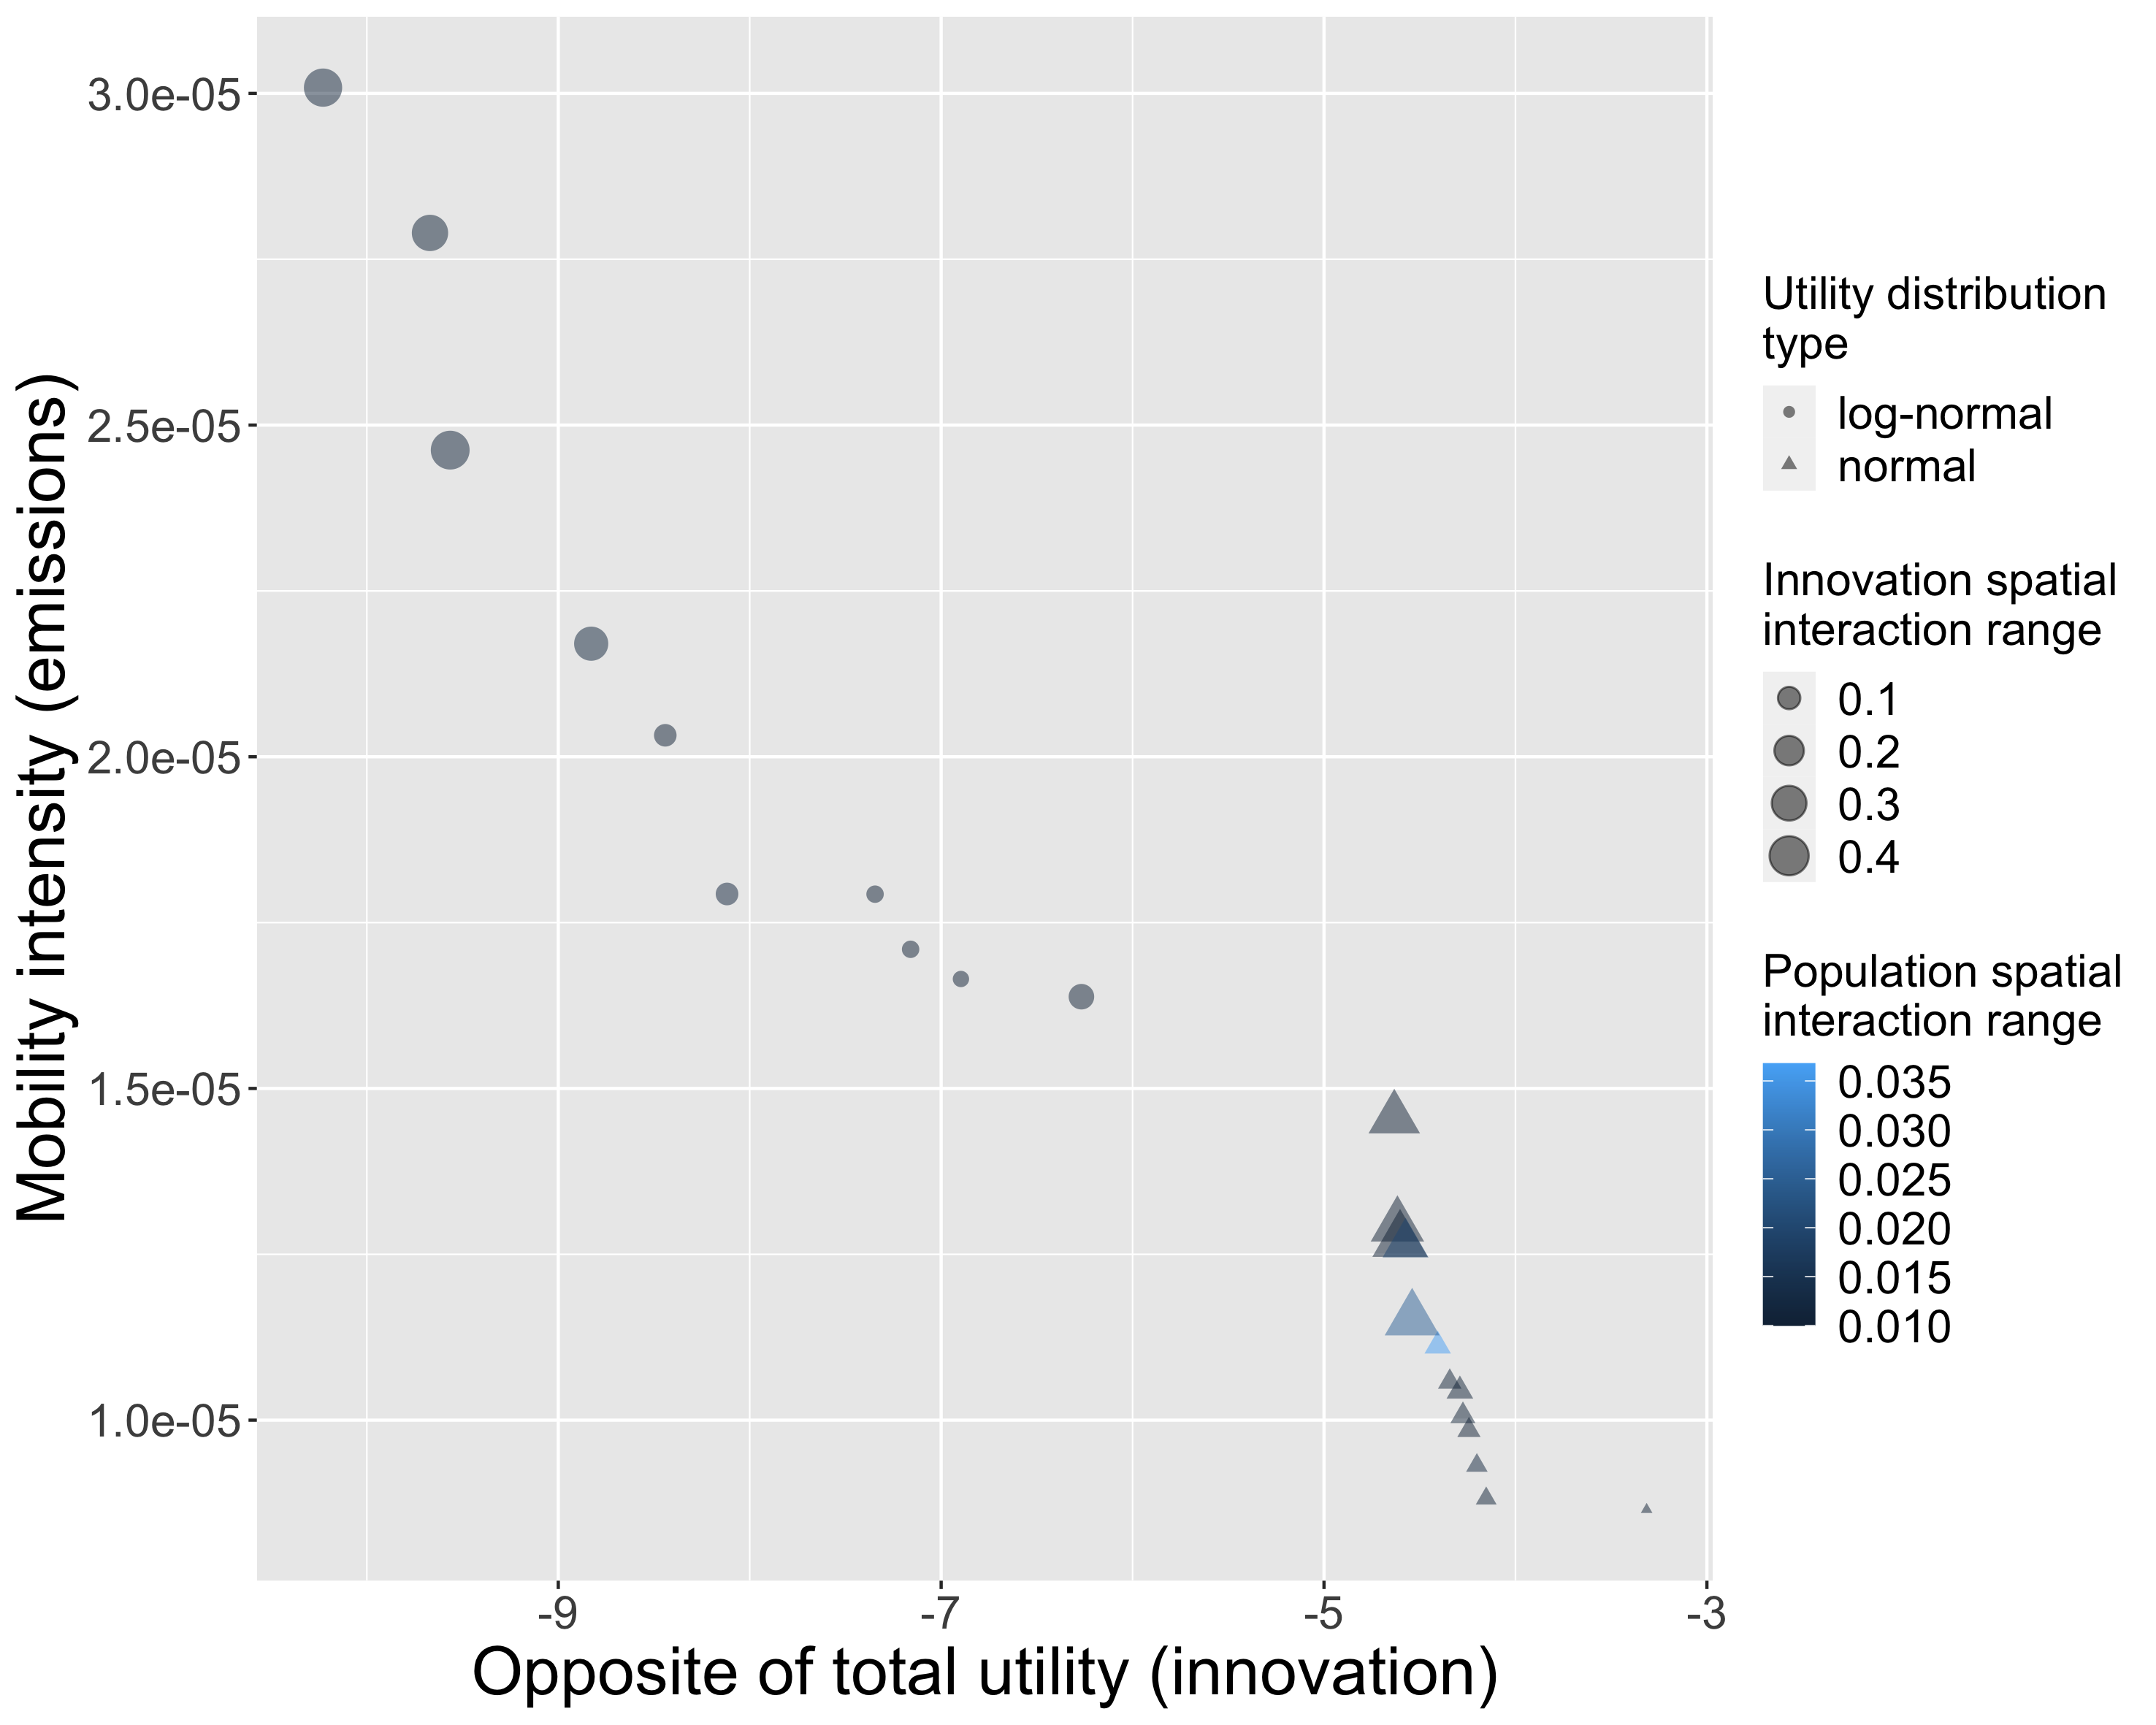
\includegraphics[height=0.7\textheight]{figures/pareto-oppAverageUtility-averageGravityFlow_color-gravityDecay_size-innovationDecay_shape-utilityDistribution.png}
\end{center}

\medskip

\textit{Pareto front confirms the existence of a trade-off}


}

\sframe{Influence of urban hierarchy}{

\begin{center}
    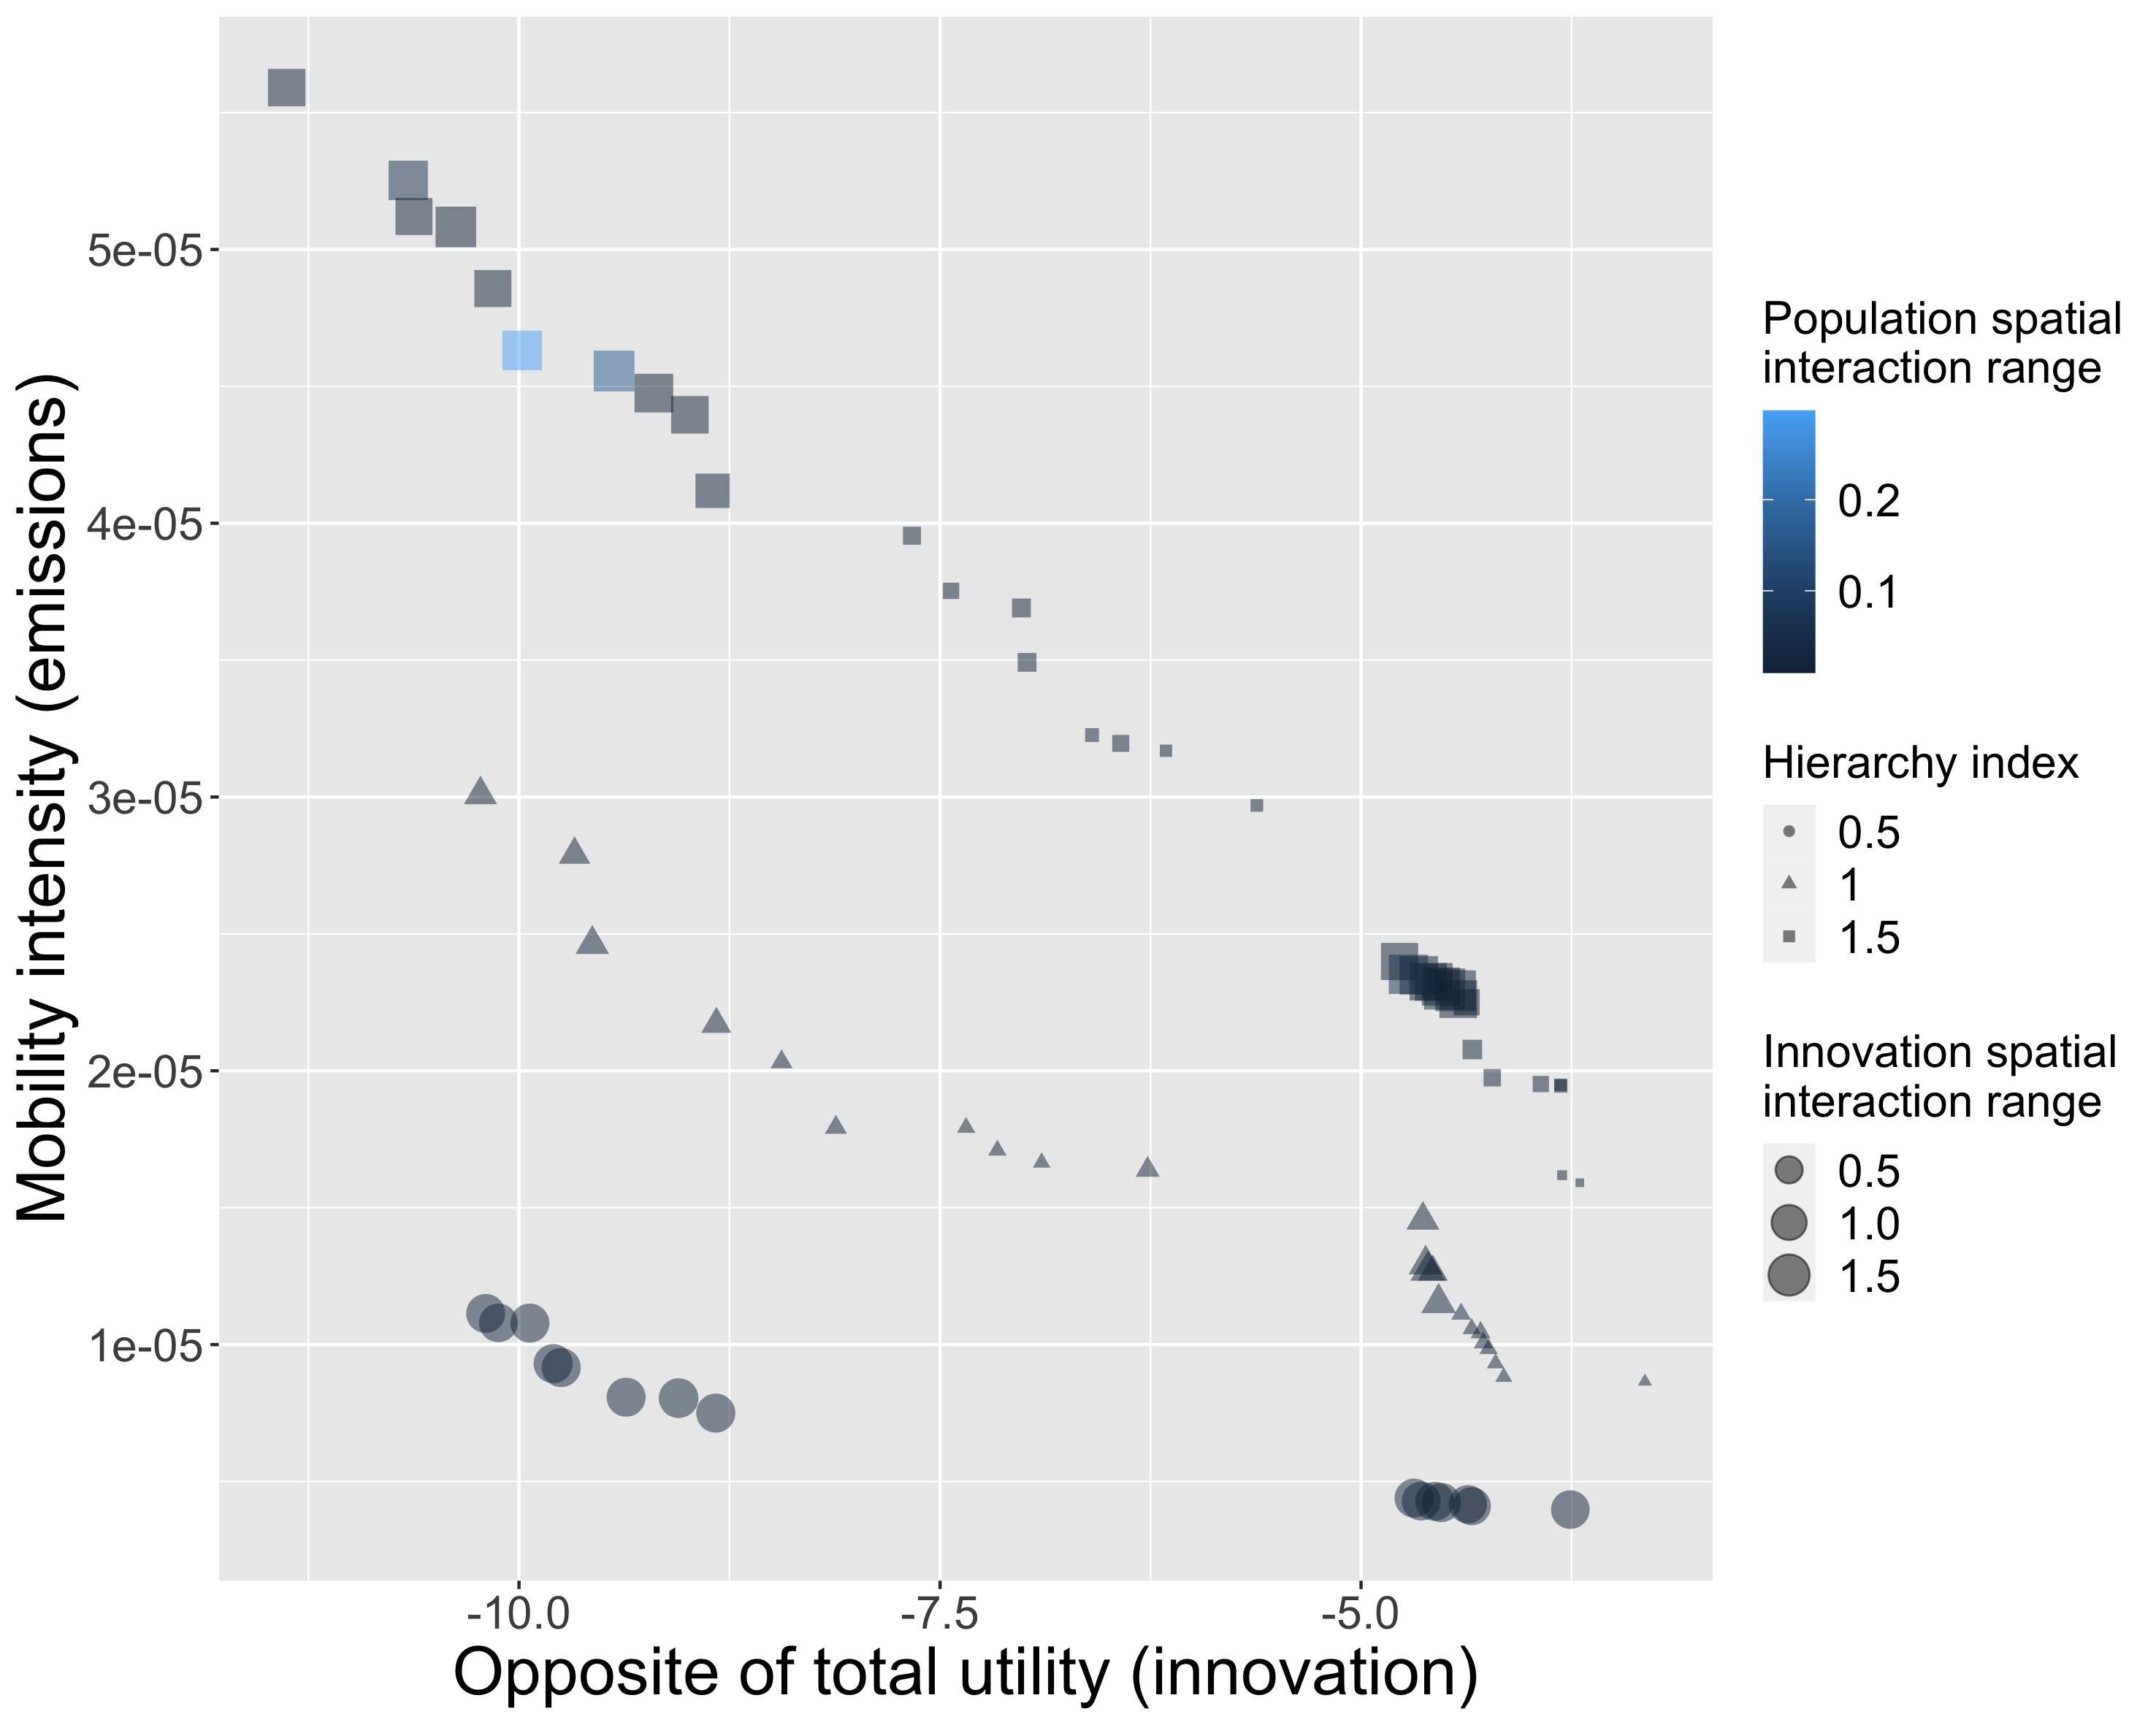
\includegraphics[height=0.7\textheight]{figures/pareto-oppAverageUtility-averageGravityFlow_VARYINGHIERARCHY_color-gravityDecay_size-innovationDecay.png}
\end{center}

\medskip

\textit{Higher inter-urban inequalities yield stronger trade-offs}



}

\sframe{Influence of innovation hierarchy}{

\begin{center}
    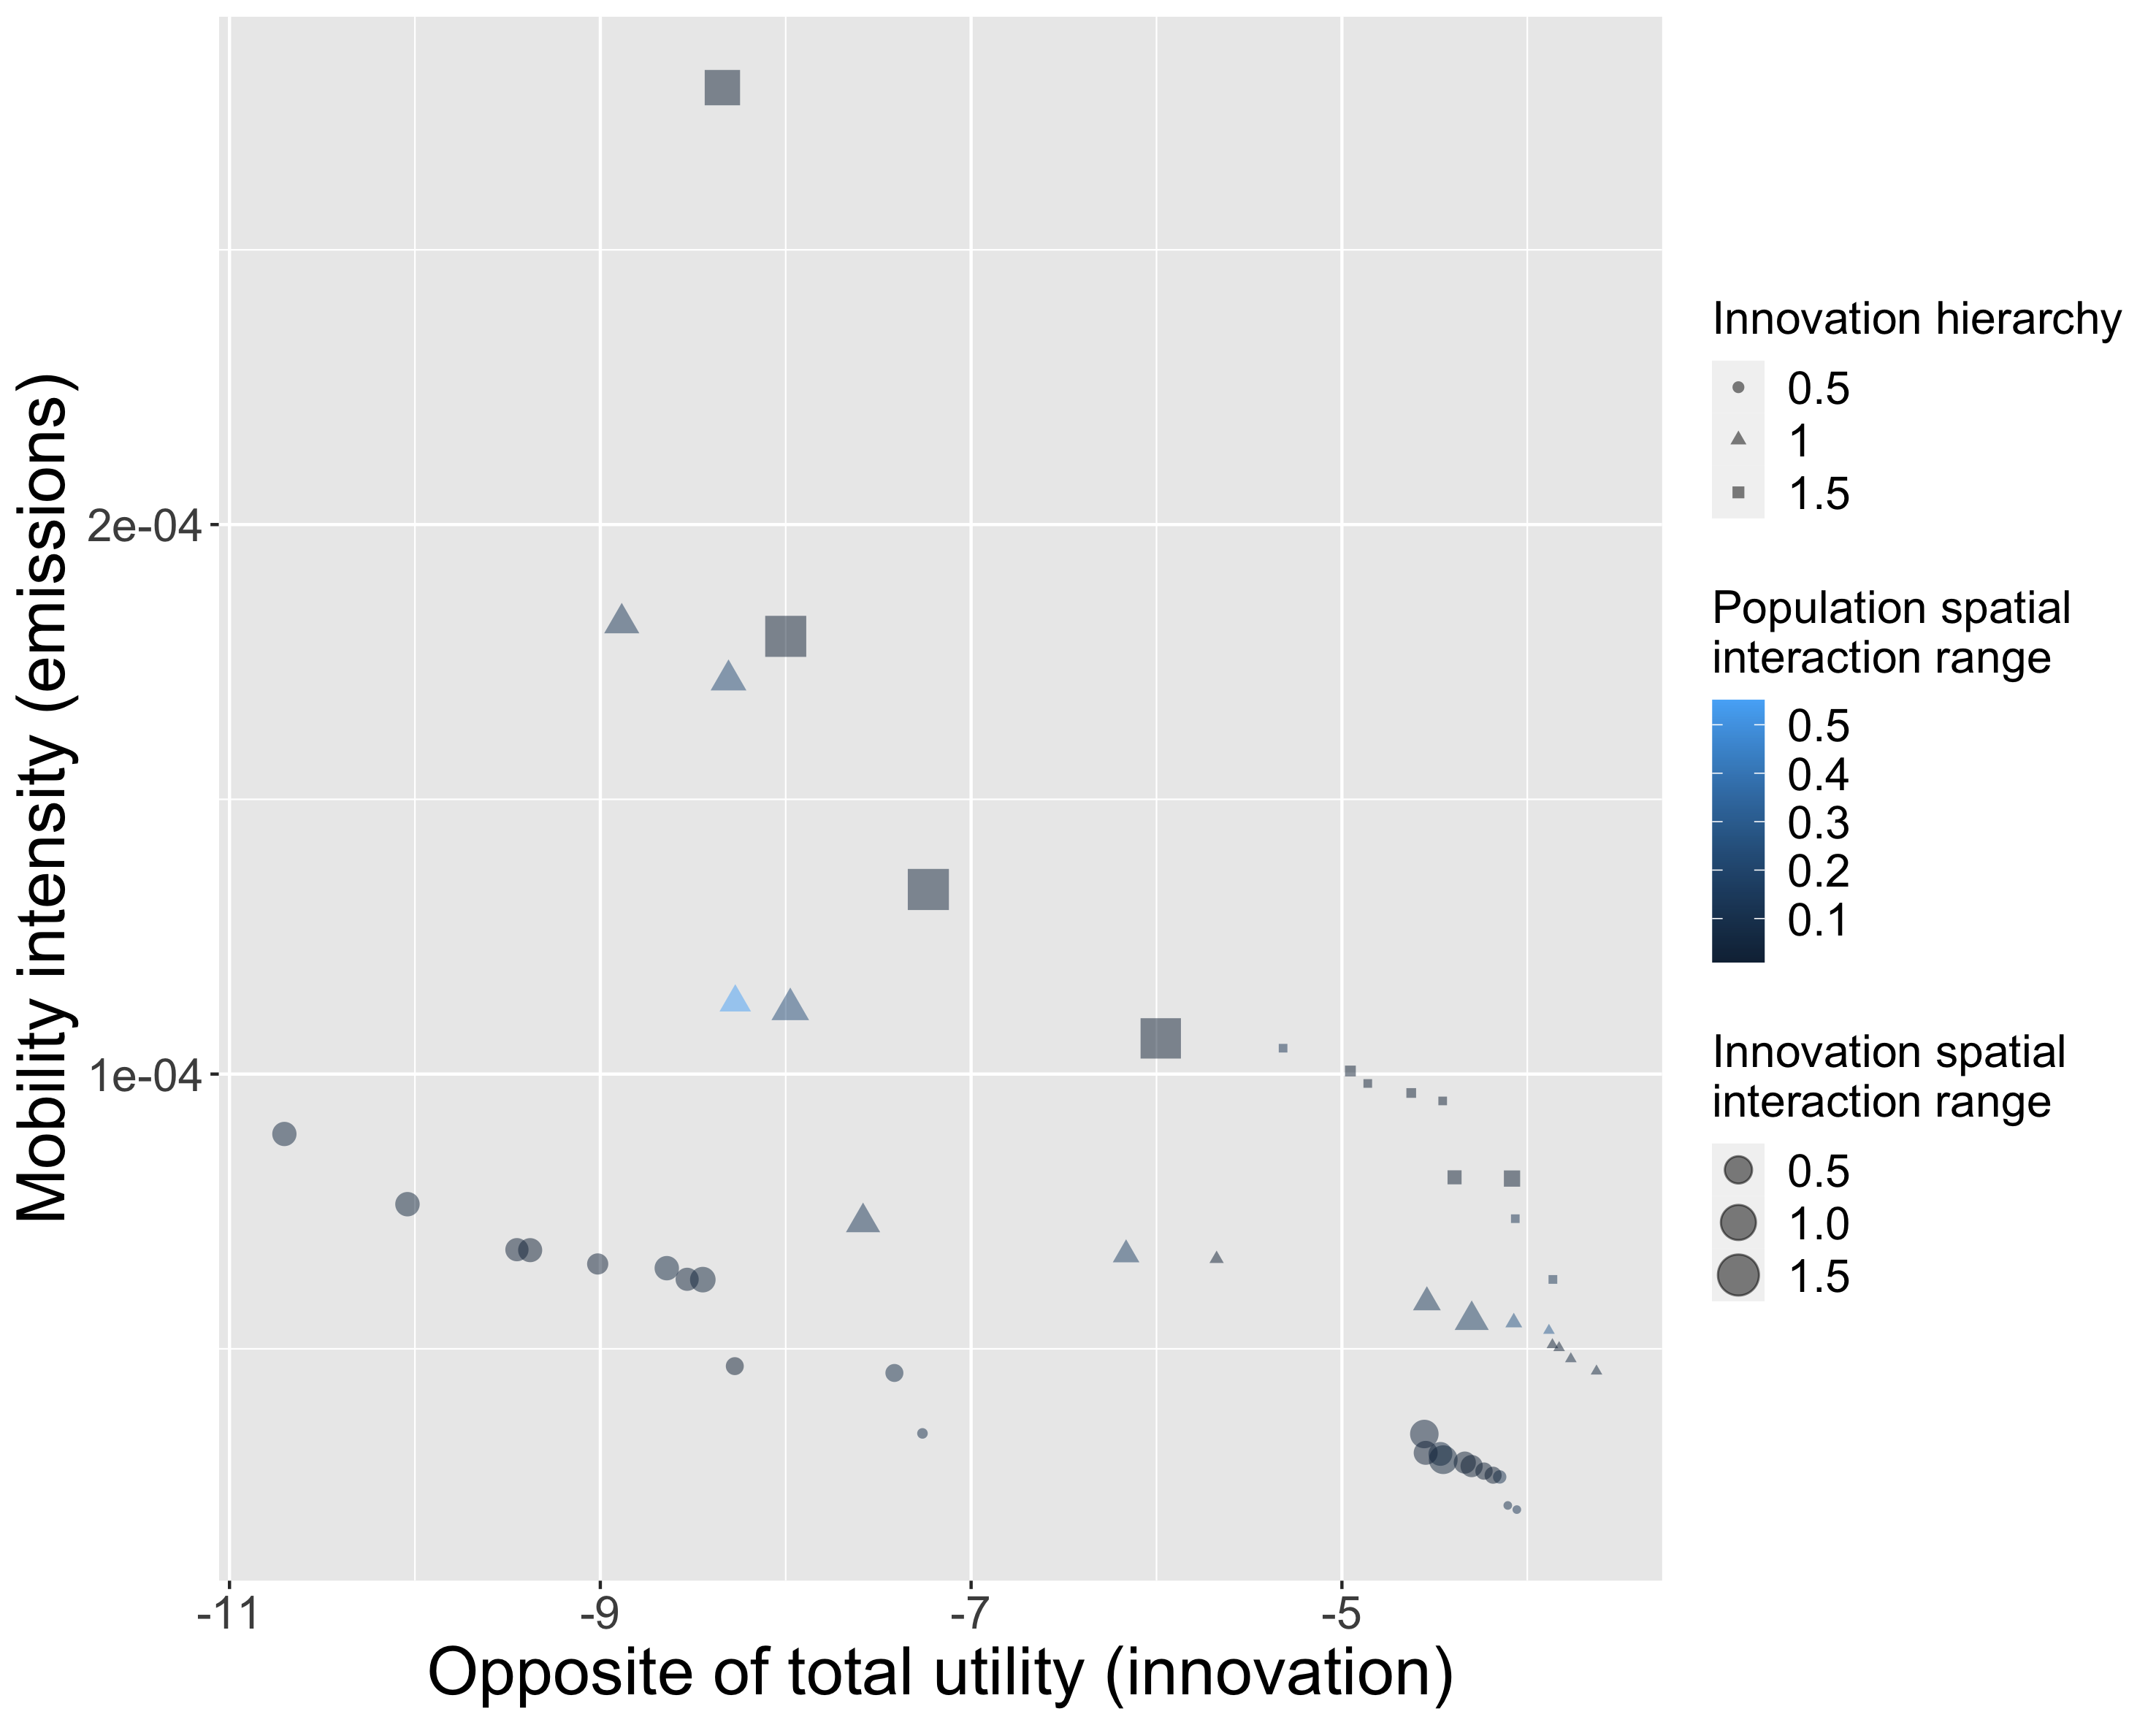
\includegraphics[height=0.7\textheight]{figures/pareto-oppAverageUtility-averageGravityFlow_VARYINGINNOVHIERARCHY_color-gravityDecay_size-innovationDecay.png}
\end{center}

\medskip

\textit{More balanced innovation yield higher utilities and less emissions (dominating Pareto front)}


}


\section{Multi-modeling}

\sframe{Generic multi-model of urban dynamics}{

\footnotesize

Other dimensions benchmarked by \cite{raimbault2020empowering} to fit population dynamics on several large urban systems


\bigskip

\textbf{Models integrated: }

\begin{itemize}
	\item Innovation diffusion urban evolution model \cite{raimbault2022trade}
	\item Marius model for economic exchanges \cite{cottineau2015modular}
	\item Co-evolution model for cities and infrastructure networks \cite{raimbault2021modeling}
\end{itemize}

\bigskip

% "semmi-weak coupling": not using workflow system - but generic

\textbf{``Semi-weak'' coupling of submodels:}

%\medskip

\begin{multline}
S_0 \rightarrow \left[ S_1^{(0)} = M_0 (S_0) \rightarrow \ldots \rightarrow S_1^{(K - 1)} = M_{K - 1} (S_1^{(K - 2)}) = S_1 \right] \longrightarrow \ldots \\
\longrightarrow \left[ S_{T}^{(0)} = M_0 (S_{T - 1}) \rightarrow \ldots \rightarrow S_T^{(K - 1)} = M_{K - 1} (S_T^{(K - 2)}) = S_T \right]
\end{multline}

\medskip

\textbf{Remarks: } strictly weak coupling does not capture dynamics nor synergies; stronger coupling may exist to better capture interdependencies processes (here no specific coupling ontology, only population and distance matrix are shared between submodels)

}

\sframe{Economic exchanges model}{

MARIUS family of models \cite{cottineau2015modular}:

\bigskip

Initial wealth as a power law of population (exponent $\alpha_W$)

\medskip

1) Update supply and demands as super-linear functions of population (exponents $\alpha_S,\alpha_D$)

\medskip

2) Exchange goods according to a gravity potential of interaction (distance decay $d_M$), supplies and demands; update wealth accordingly

\medskip

3) Update population such that population difference is a power law of wealth difference (economic multiplier $e_M$ and exponent $\alpha_P$)


}


\sframe{Infrastructure co-evolution model}{

\textit{System of cities interaction model including network evolution.}

\medskip

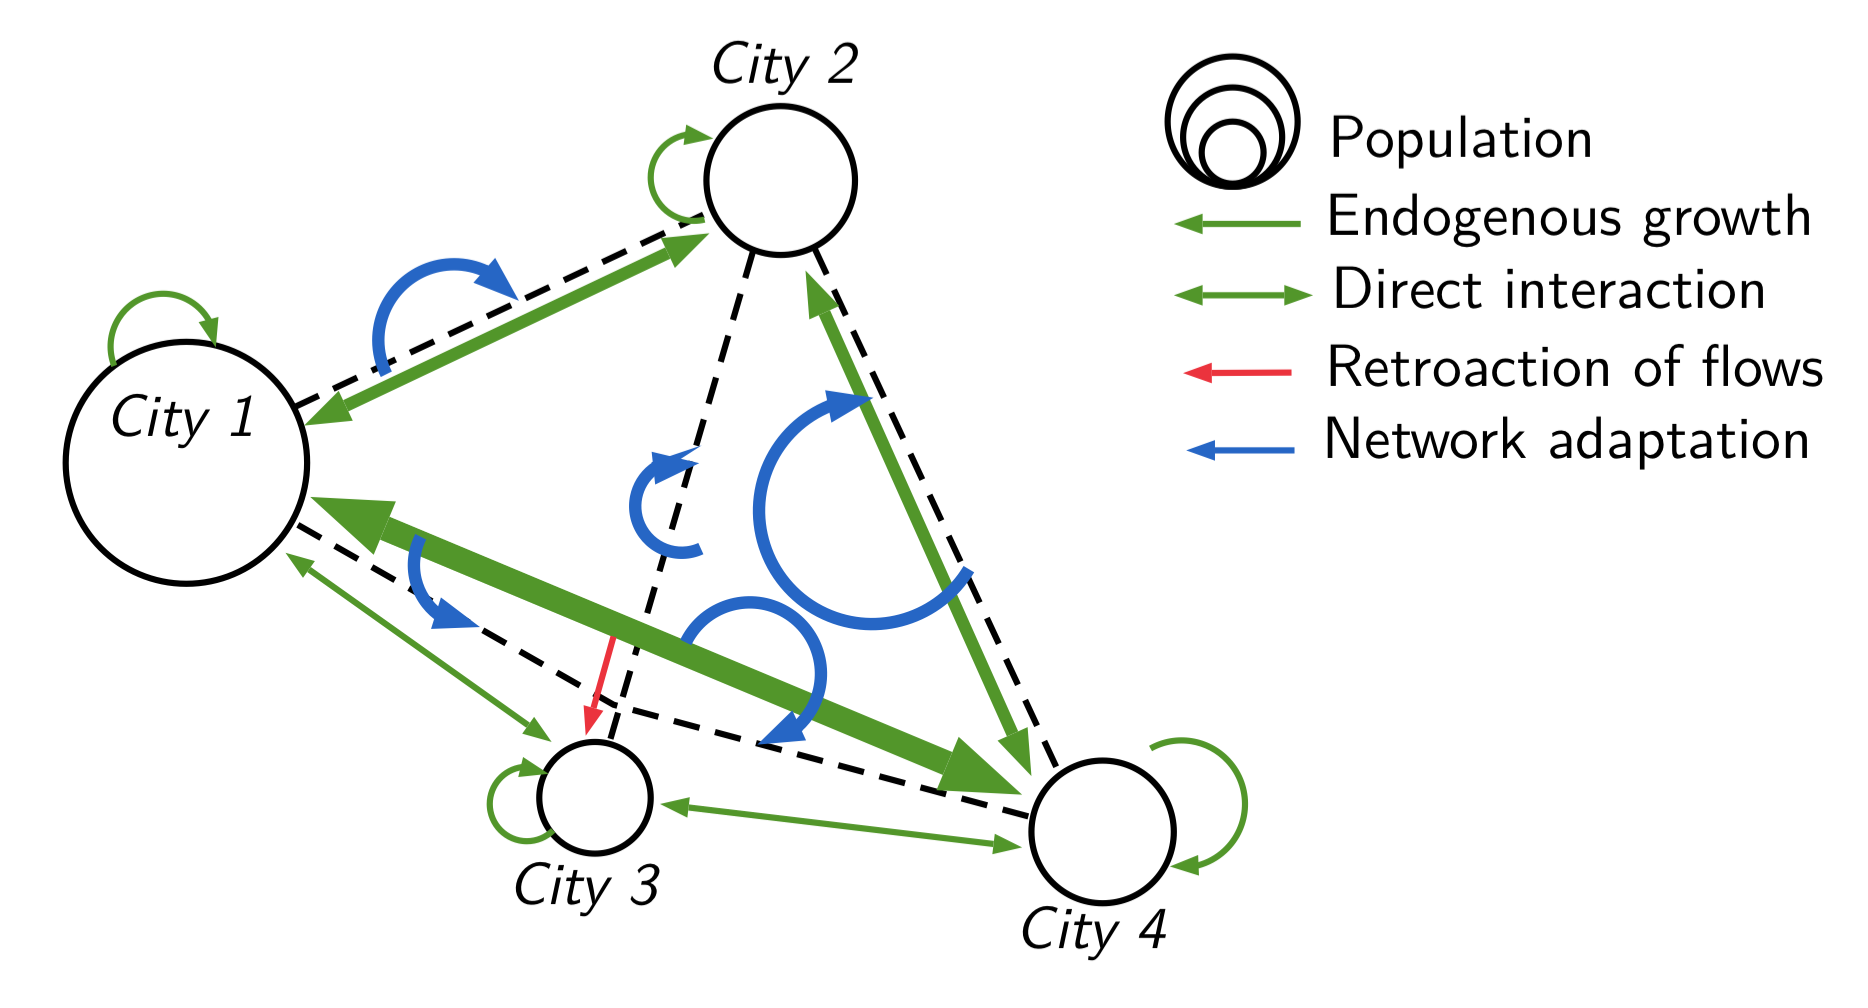
\includegraphics[width=0.6\textwidth]{figures/macrocoevol_en.png}
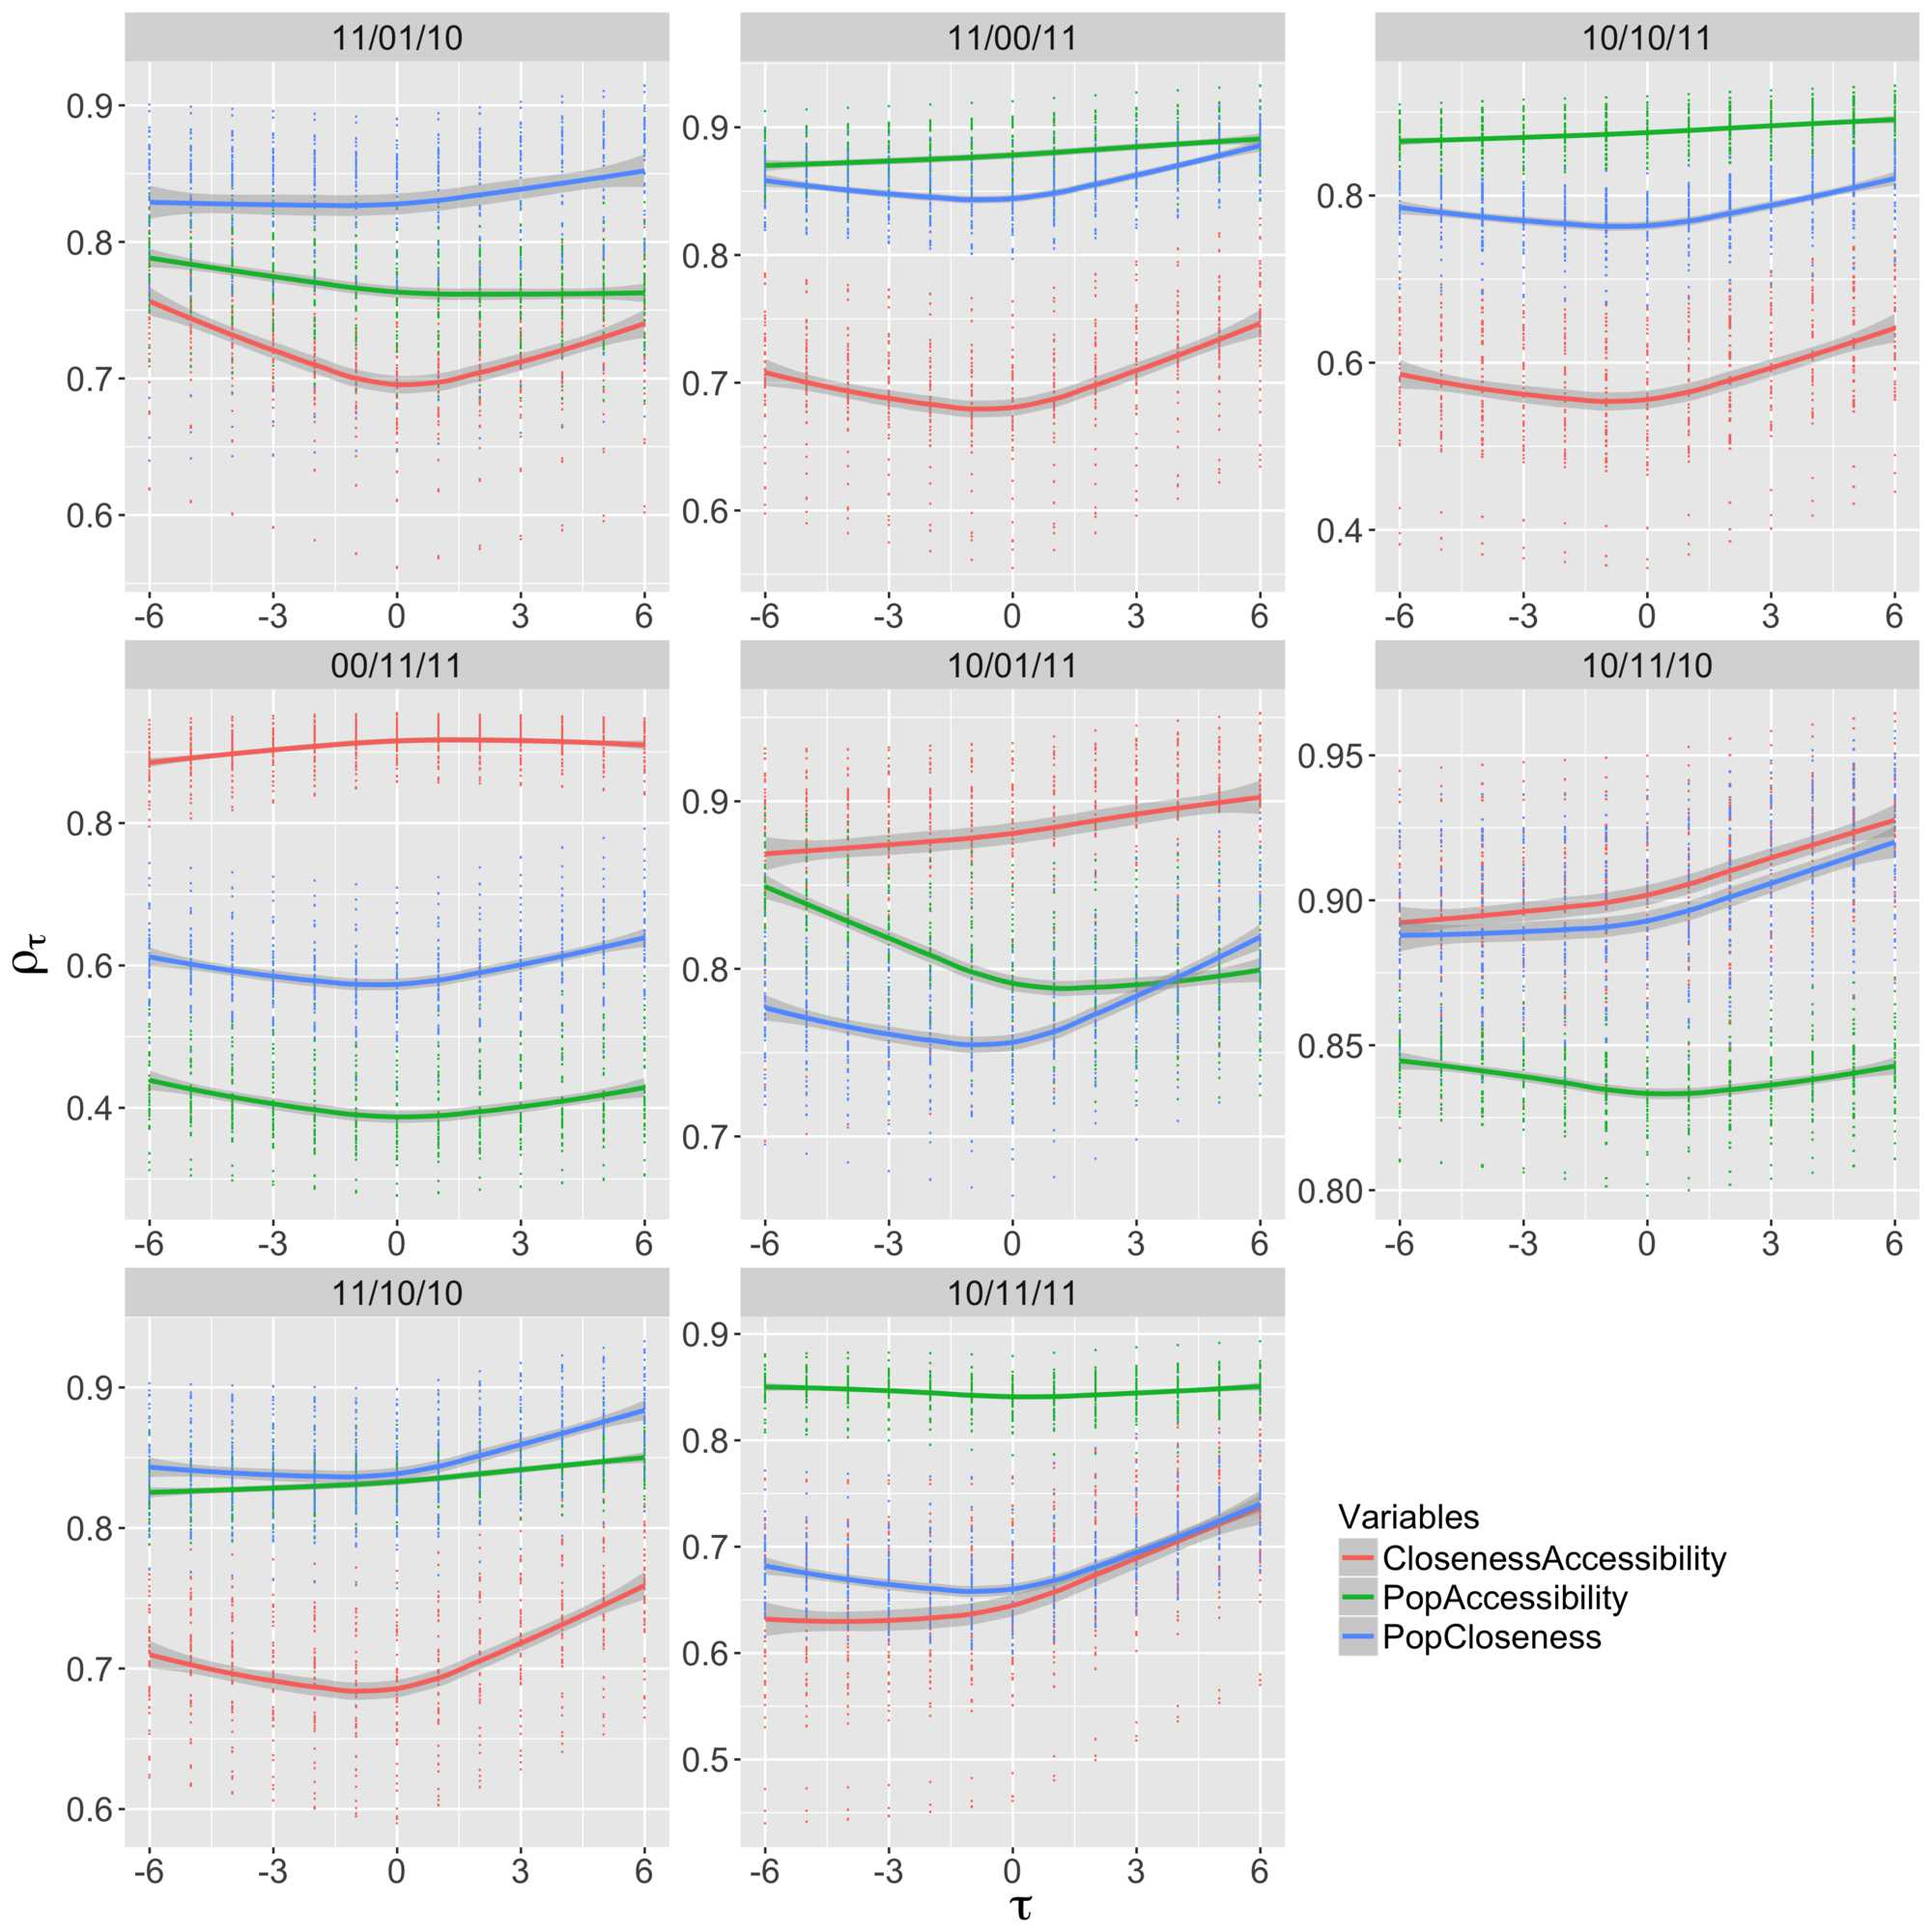
\includegraphics[width=0.39\linewidth]{figures/6-2-2-fig-macrocoevol-correlations.jpg}


\nocite{raimbault2020indirect}
\nocite{raimbault2021modeling}
\nocite{raimbault2022hierarchy}

\bigskip

\tiny

Raimbault, J. (2020). Indirect evidence of network effects in a system of cities. Environment and Planning B: Urban Analytics and City Science, 47(1), 138-155.

\smallskip

Raimbault, J. (2021). Modeling the co-evolution of cities and networks. In Handbook of Cities and Networks (pp. 166-193). Edward Elgar Publishing.

\smallskip

Raimbault, J. (2020). Hierarchy and co-evolution processes in urban systems. Forthcoming in Hierarchy in infrastructure networks, J. Fen-Chong, ed. ISTE Editions.


}

\sframe{Optimised objectives}{

\textbf{Proxies for SDGs:}

\medskip

\begin{itemize}
	\item Total utility of innovations (SDG 9 ``Innovation'')
	\item Total spatial interaction flows across submodels (SDG 13 ``Climate'')
	\item Average distance between cities (SDG 9 ``Resilient infrastructure'')
	\item Economic inequalities (SDG 10 ``Inequalities'')
	\item Total wealth of cities (SDG 8 ``Economic Growth'')
\end{itemize}

\bigskip

\textbf{Optimisation parameters: } fixed synthetic urban system parameters but random configurations (10 repetitions); 8 parameters for innovation; 6 parameters for economic exchanges; 6 parameters for co-evolution



}


\sframe{Optimisation results}{


\begin{center}
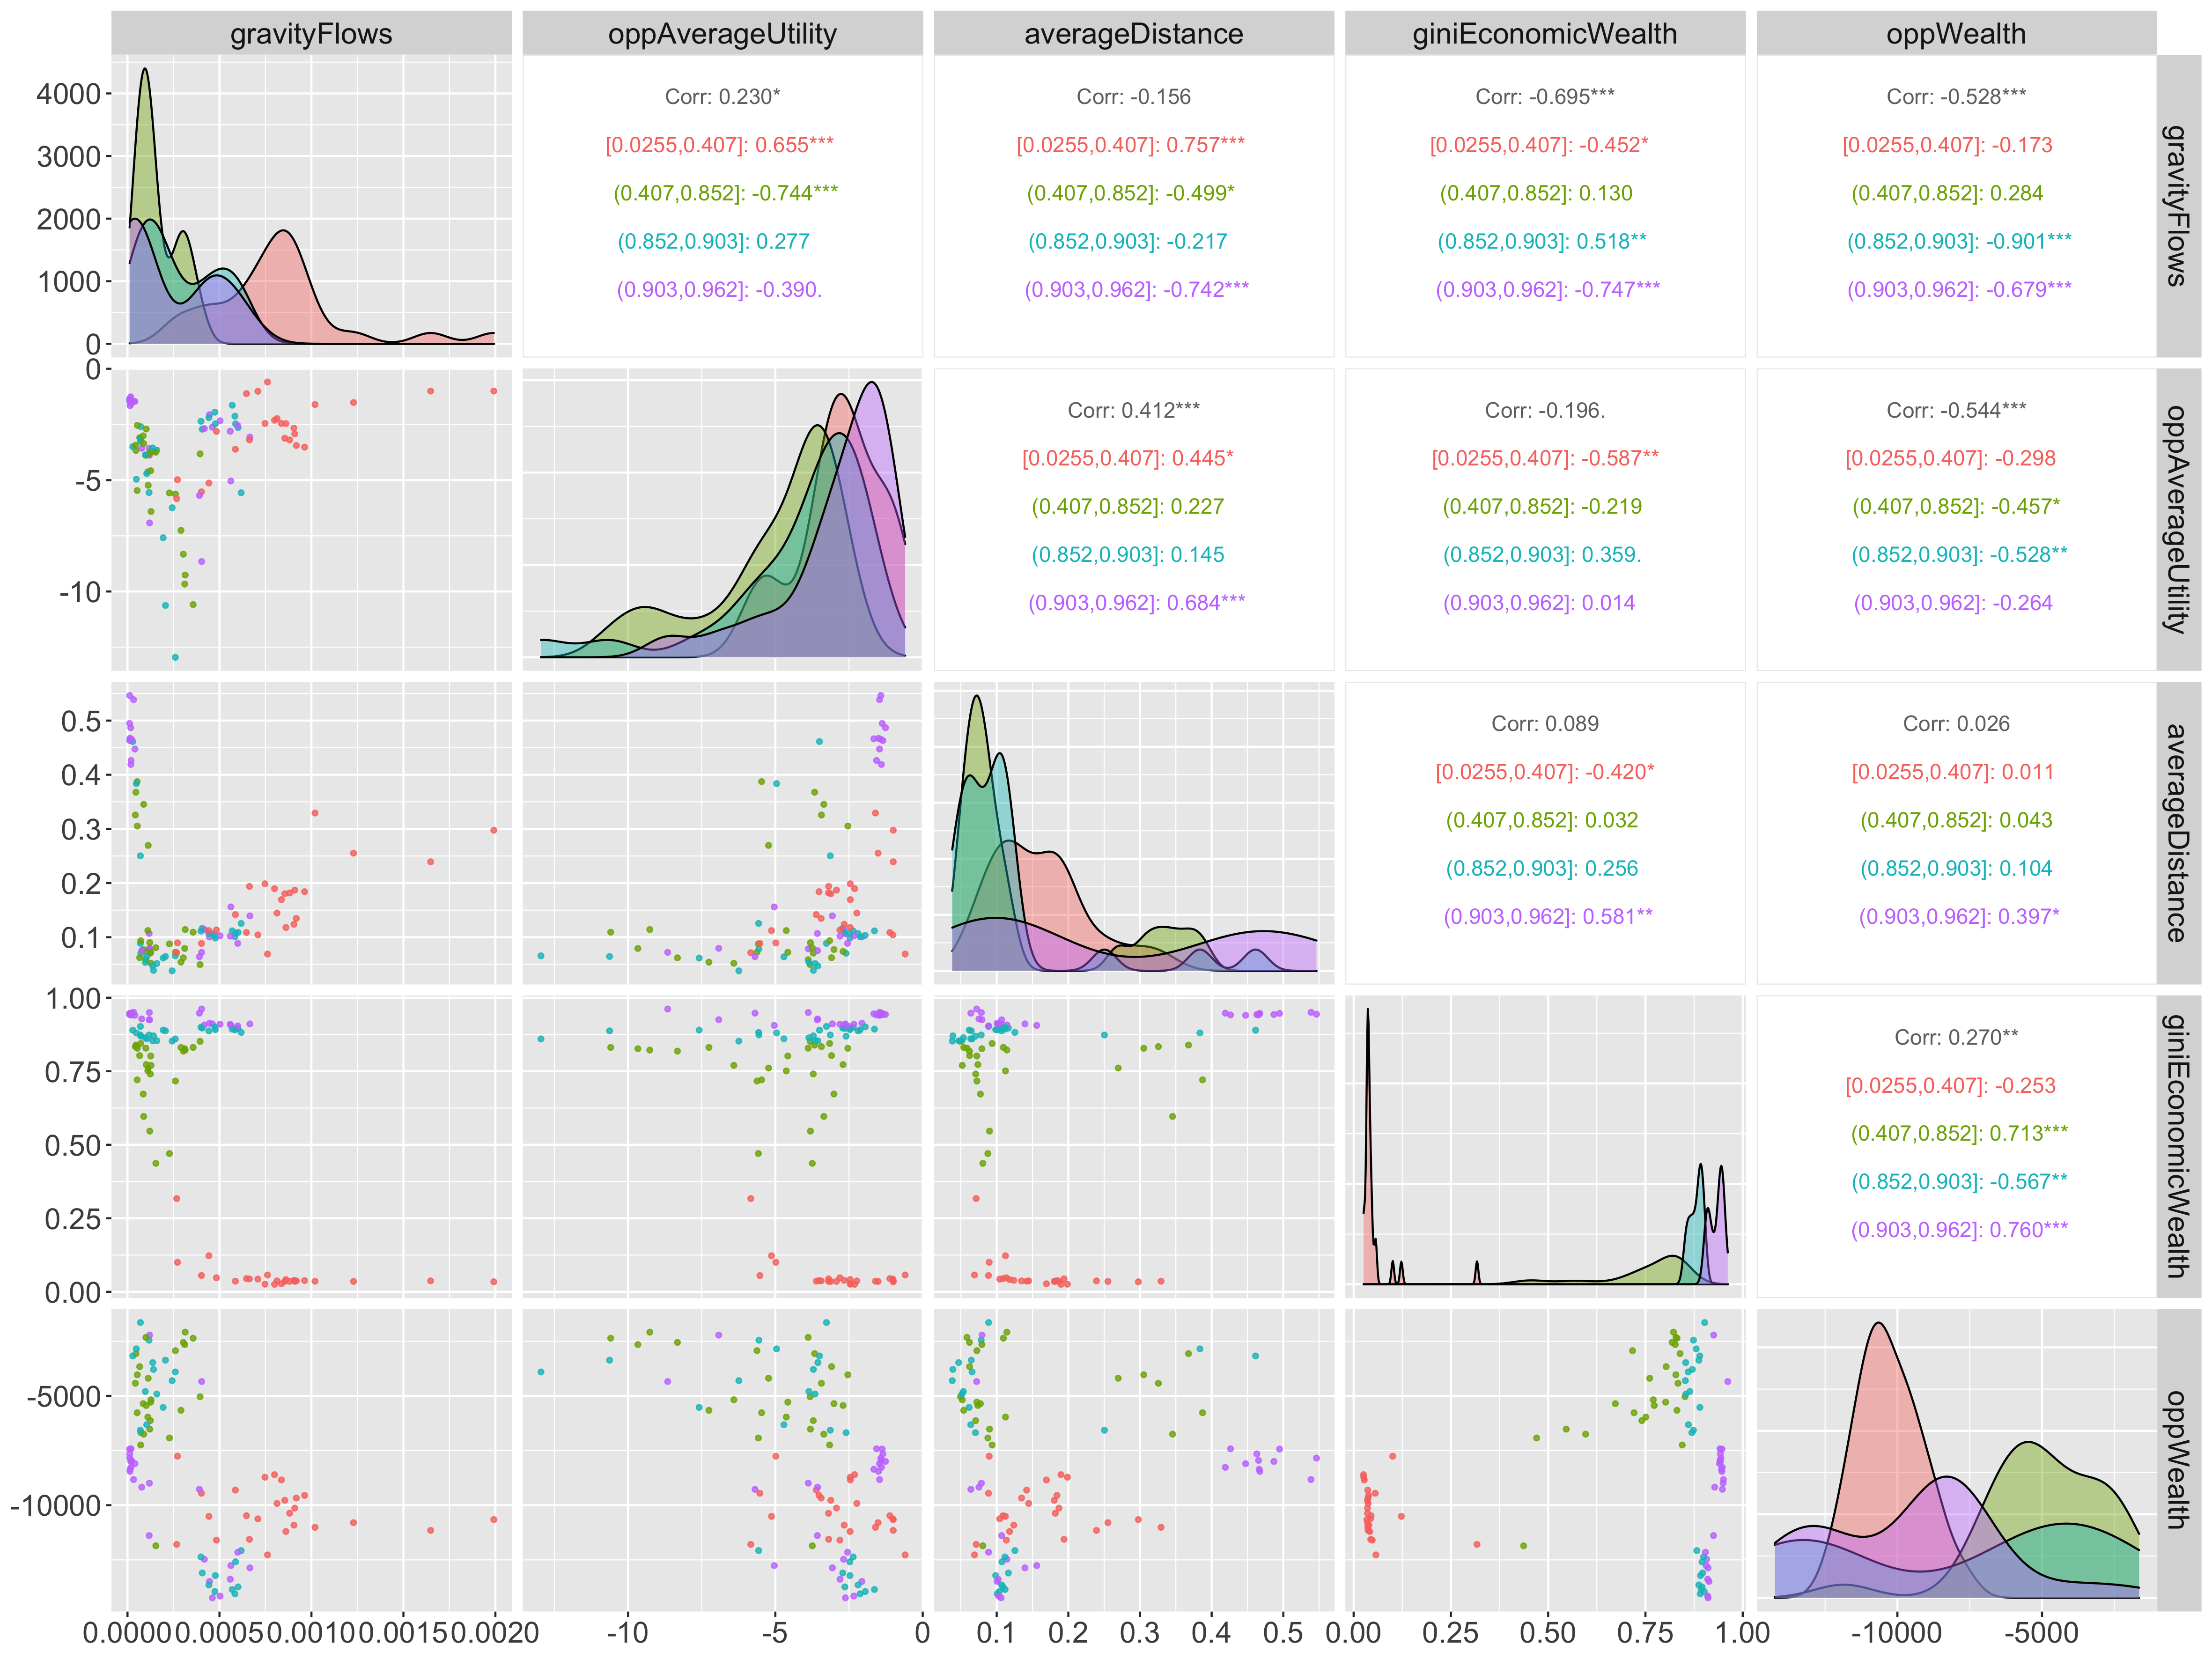
\includegraphics[width=0.86\linewidth]{figures/scatter_models_colorginiEconomicWealth_OPTIMISATION_GRID_20220622_092133.png}
\end{center}

\footnotesize
\textit{Scatterplots of the 5D Pareto front. Color level: Gini economic wealth.}

}

\sframe{Optimisation results}{


\begin{center}
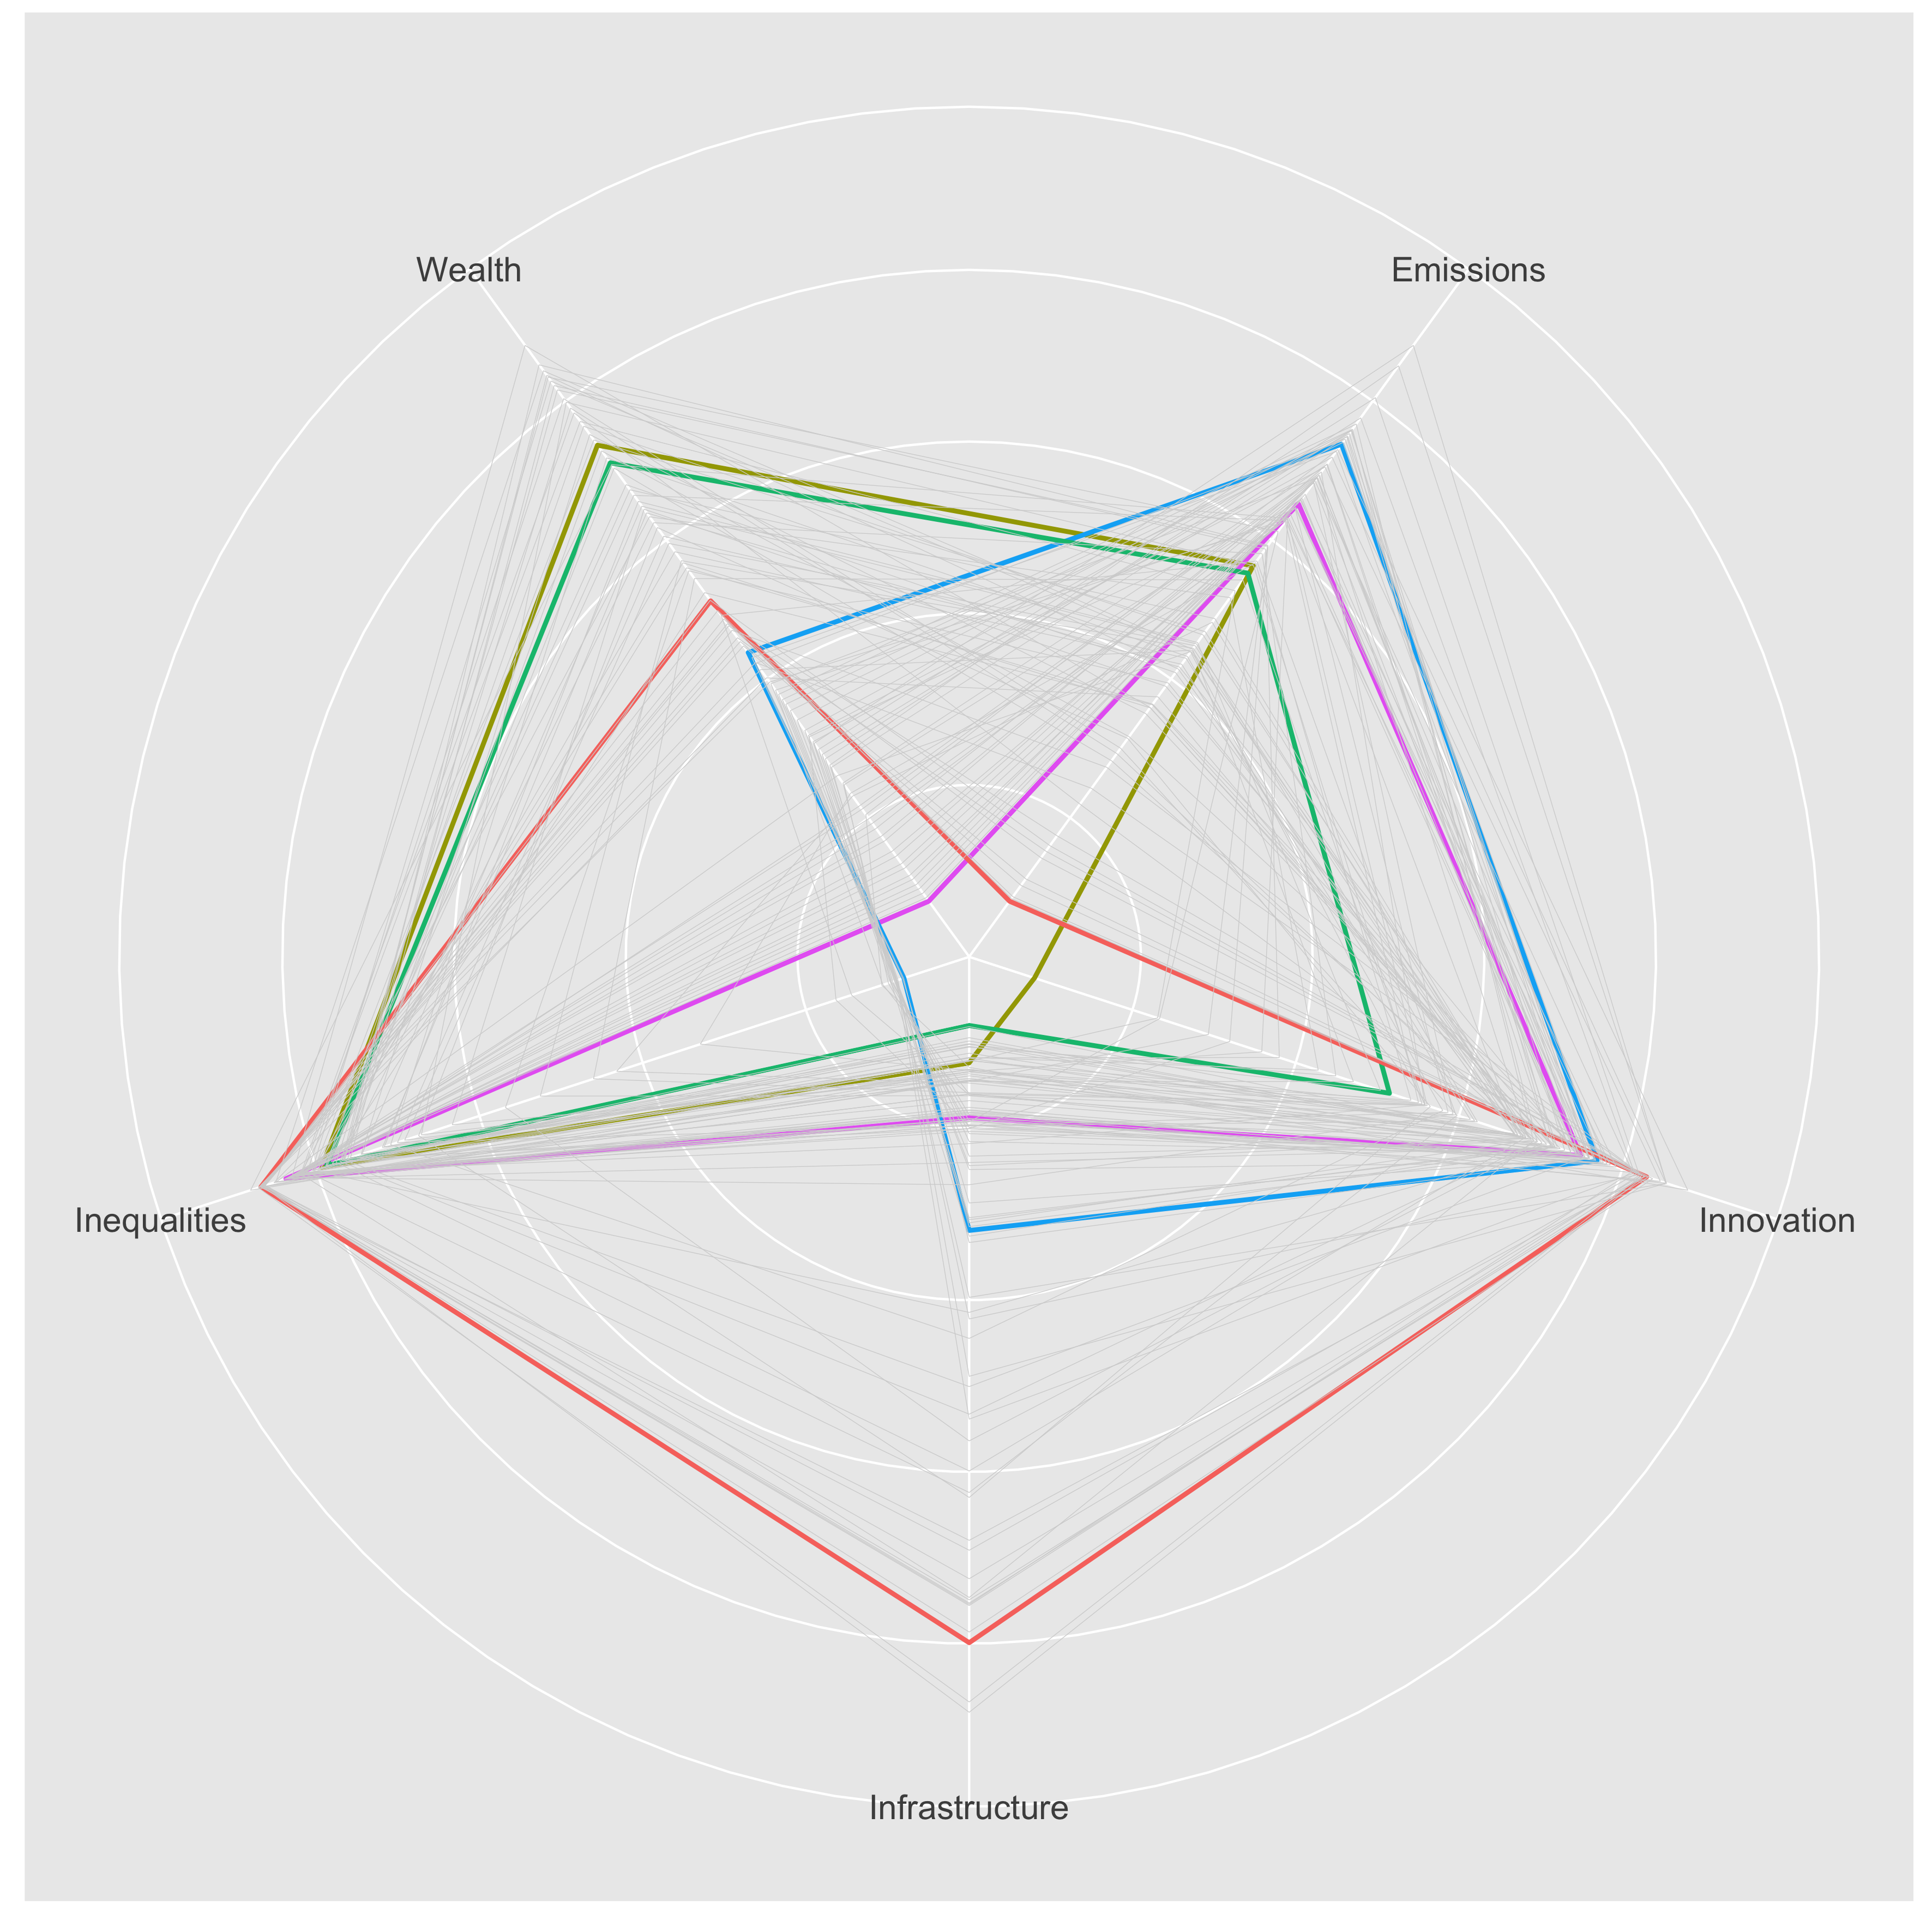
\includegraphics[width=0.65\linewidth]{figures/radar_sdgs.png}
\end{center}

\tiny
\textit{Radar plot for the many-objective optimisation (colour: best solution along each dimension)}

}





\section{Discussion}


\sframe{Discussion}{

\footnotesize

\textbf{Parametrisation on case studies:}

\medskip

$\rightarrow$ Patent data as a proxy for innovation: geolocation of inventors not straightforward \cite{bergeaud2021patentcity} \cite{de2019geocoding}; which technological (sub-)classes? Model with one dimension (extension with a matrix genome?); semantic content to better capture innovation diffusion? \cite{bergeaud2017classifying}

\medskip

$\rightarrow$ Emissions: inter-urban mobility emissions difficult to capture (need an additional transport model?)

\medskip

$\rightarrow$ Historical infrastructure networks data?

\bigskip

\textbf{Work in progress}

\medskip

$\rightarrow$ Many-objective optimisation: NSGA3 algorithm

\medskip

$\rightarrow$ Empirical stylised facts on possible trade-offs in systems of cities

\bigskip


\textbf{Future work}

\medskip

$\rightarrow$ Towards multi-scale models: quantifying goal 11 (sustainable cities and communities) implies in some cases intra-urban dynamics (mobility, segregation, e.g.)

\medskip

$\rightarrow$ Transfer to policies and planning? Models with multiple functions? \cite{varenne2018theories} (towards companion modeling and stakeholder involvement)


}







\section{Conclusion}


\sframe{Conclusion}{

$\rightarrow$ Towards an integrative urban and territorial science applied to sustainable planning at multiple scales

\medskip

$\rightarrow$ Transfer to decision-making, policies and governance? \textit{e-team} of the CSDC campus





\bigskip
\bigskip
\bigskip

\textbf{To use OpenMOLE (free and open software) and contribute: }\\
\url{https://openmole.org}

\bigskip

\textbf{Model code and results open source at }

\url{https://github.com/JusteRaimbault/SDGTradeoffs} and

\url{https://github.com/openmole/spatialdata}

}









%%%%%%%%%%%%%%%%%%%%%
\begin{frame}[allowframebreaks]
\frametitle{References}
\bibliographystyle{apalike}
\bibliography{biblio}
\end{frame}
%%%%%%%%%%%%%%%%%%%%%%%%%%%%





\end{document}



